% For more detailed article preparation guidelines, please see: http://wellcomeopenresearch.org/for-authors/article-guidelines and http://wellcomeopenresearch.org/for-authors/data-guidelines

\documentclass[10pt,a4paper,twocolumn]{article}
\usepackage{WellcomeOR_styles}

%% Packages added manually
\usepackage{float}
\usepackage{hyperref}
\usepackage{booktabs}
\usepackage{longtable}


%% Default: numerical citations
\usepackage[numbers]{natbib}

%% Uncomment this lines for superscript citations instead
% \usepackage[super]{natbib}

%% Uncomment these lines for author-year citations instead
% \usepackage[round]{natbib}
% \let\cite\citep

\begin{document}

\title{Human Judgement Forecasting of COVID-19 in the UK}
%\titlenote{The title should be detailed enough for someone to know whether the article would be of interest to them, but also concise. Please ensure the broadness and claims within the title are appropriate to the content of the article itself.}


\author[1, 2, 3]{Nikos I. Bosse}
\author[1, 2]{Sam Abbott}
\author[6, 7]{Johannes Bracher}
\author[1, 4]{Edwin van Leeuwen}
\author[5]{Anne Cori}
\author[1, 2, 3]{Sebastian Funk}


\affil[1]{Department of Infectious Disease Epidemiology, London School of Hygiene \& Tropical Medicine, London, United Kingdom}
\affil[2]{Centre for the Mathematical Modelling of Infectious Diseases, London, United Kingdom}
\affil[3]{NIHR Health Protection Research Unit in Modelling \& Health Economics}
\affil[4]{Modelling Economics Unit and NIHR Health Protection Research Unit in Modelling \& Health Economics, UK Health Security Agency, London, United Kingdom}
\affil[5]{MRC Centre for Outbreak Analysis and Modelling, Department of Infectious Disease Epidemiology, School of Public Health, Imperial College London, London, United Kingdom}
\affil[6]{Chair of Statistical Methods and Econometrics, Karlsruhe Institute of Technology, Karlsruhe, Germany}
\affil[7]{Computational Statistics Group, Heidelberg Institute for Theoretical Studies, Heidelberg, Germany}

\maketitle
\thispagestyle{fancy}

% Please list all authors that played a significant role in the research involved in the article. Please provide full affiliation information (including full institutional address, ZIP code and e-mail address) for all authors, and identify who is/are the corresponding author(s).



\begin{abstract}
%Abstracts should be up to 300 words and provide a succinct summary of the article. Although the abstract should explain why the article might be interesting, care should be taken not to inappropriately over-emphasise the importance of the work described in the article. Citations should not be used in the abstract, and the use of abbreviations should be minimized. If you are writing a Research or Systematic Review article, please structure your abstract into Background, Methods, Results, and Conclusions.

\paragraph{Background}

Accurate forecasts of infectious diseases can aid public health decision-making. In the past, two studies found ensembles of human judgement forecasts of COVID-19 to show predictive performance comparable to ensembles of computational models, at least when predicting case incidences. We present a follow-up to a study conducted in Germany and Poland and investigate a novel joint approach to combine human judgement and epidemiological modelling. 

\paragraph{Methods}

From May 24th to August 16th 2021, we elicited weekly one to four-week-ahead forecasts of cases and deaths from COVID-19 in the UK from a crowd of human forecasters. Forecasts were elicited as part of a tournament, the "UK Crowd Forecasting Challenge", and a median ensemble of all forecasts was submitted to the European Forecast Hub. Participants could use two distinct interfaces: in one, forecasters submitted a predictive distribution directly, in the other forecasters instead submitted a forecast of the effective reproduction number $R_t$ based on an estimated baseline. This was then used to forecast cases and deaths using simulation methods from the \texttt{EpiNow2} \textsf{R} package. Forecasts were scored using the weighted interval score on the original forecasts, as well as after applying the natural logarithm to both forecasts and observations. 

\paragraph{Results}

The ensemble of human forecasters overall performed comparably to the official European Forecast Hub ensemble on both cases and deaths, although results were susceptible to changes in details of the evaluation. $R_t$ forecasts performed comparably to direct forecasts on cases, but worse on deaths. Self-identified experts did not outperform non-experts though the sample size was small. 

\paragraph{Conclusions}

Human judgement can be useful in predicting the spread of an infectious disease such as COVID-19. The results of forecast evaluations can change depending on what metrics are chosen and judgement on what does or doesn't constitute a "good" forecast is dependent on the forecast consumer. Combinations of human and computational forecasts hold potential but present real-world challenges that need to be solved.



\end{abstract}

\section*{Keywords}

Human judgement forecasting, COVID-19, infectious disease, 

% Please list up to eight keywords to help readers interested in your article find it more easily.


\clearpage

\section*{Introduction}

Infectious disease modelling and forecasting has attracted wide-spread attention during the COVID-19 pandemic and helped inform decision making in public health organisations and governments \cite{cramerEvaluationIndividualEnsemble2021, venkatramananUtilityHumanJudgment2022}. 
% Beginning in March 2020, forecasts for different COVID-19 targets have been systematically collated by Forecast Hubs in the US \citep{cramerEvaluationIndividualEnsemble2021}, Germany and Poland \citep{bracherShorttermForecastingCOVID192021, bracherNationalSubnationalShortterm2021}, and Europe \citep{sherrattPredictivePerformanceMultimodel2022a}. 
Most forecasts used to inform decision making were based on computational models of COVID-19, but some authors also explored human judgement forecasting as an alternative or in combination \cite{recchiaHowWellDid2021, mcandrewExpertJudgmentModel2022, bosseComparingHumanModelbased2022, mcandrewChimericForecastingCombining2022}. 

Past research found that in the context of infectious disease forecasting, human judgement forecasts could achieve predictive performance broadly comparable to forecasts generated based on mathematical modelling, in particular when forecasting incident cases. \citet{farrowHumanJudgmentApproach2017} found that an aggregate of human predictions outperformed computational models when predicting the 2014/15 and 2015/16 flu season in the US. However, a comparable approach performed worse than computational models at predicting the 2014/15 outbreak of chikungunya in the Americas. 
\citet{bosseComparingHumanModelbased2022} found an ensemble of human forecasters to outperform an ensemble of computational models when predicting cases of COVID-19 in Germany, but performing worse when predicting incident deaths. Similarly, \citet{mcandrewChimericForecastingCombining2022} reported an ensemble of human forecasters to perform comparably to an ensemble of computational models when predicting incident cases, and worse when predicting incident deaths. \citet{farrowHumanJudgmentApproach2017} and in particular \citet{bosseComparingHumanModelbased2022} struggled to recruit a large number of participants (numbers of active forecasters ranged from 22 to 61 in \citet{mcandrewChimericForecastingCombining2022}, 7 to 24 in \citet{farrowHumanJudgmentApproach2017}, and 4 to 10 in \citet{bosseComparingHumanModelbased2022}). 
It is important to note that in previous studies (and also this one) human forecasters were free to use any resources, including computational models, in the process of creating a forecast, making it difficult to completely separate human judgement and computational modelling. 

In some situations, human judgement forecasting may have advantages relative to computational models. Human judgment may be particularly useful to provide timely forecasts in situations where data is sparse and many parameters are unknown. Humans are generally able to answer a broad set of question (such as for example the likelihood that a given actor will take some specified action) or can take factors into account that are hard to encode in a computational model. On the other hand, human judgement forecasting is difficult to scale due to the time and effort required, and humans may be at a disadvantage at tasks that strongly benefit from the ability to perform complex computations. Also, the use of human judgement forecasts by decision makers may be complicated by the lack of clarity of the basis on which they were made.

% Beginning in March 2020, forecasts for different COVID-19 targets have been systematically collated by Forecast Hubs in the US \citep{cramerEvaluationIndividualEnsemble2021}, Germany and Poland \citep{bracherShorttermForecastingCOVID192021, bracherNationalSubnationalShortterm2021}, and Europe \citep{sherrattPredictivePerformanceMultimodel2022a}. 

Methods that aim to combine human judgement and mathematical modelling are therefore appealing, though we note that presenting this as a binary choice is misleading as most computational models in use in epidemiology have at least some element of human judgement supporting their structure or usage and many human forecasters make use of simple base rate based approaches which are in reality simple models. One explicit method to combine separate human judgement and computational model forecasts with the goal of improving predictive performance is an ensemble. This has been widely shown to improve performance across model types \citep{mcandrewChimericForecastingCombining2022}. \citet{farrowHumanJudgmentApproach2017, bosseComparingHumanModelbased2022, swallowChallengesEstimationUncertainty2022} and others suggested additional possibilities in the context of infectious diseases that may also help reduce the amount of human effort required. One approach is to use human forecasts, for example of relevant disease parameters, as an input to computational modelling. Another approach is to use mathematical modelling in explicit combination with human judgement, for example by giving experts the option to make post-hoc adjustments to model outputs. \citet{bosseComparingHumanModelbased2022} proposed asking human forecasters to forecast the effective reproduction number $R_t$ (the average number of people an infected person would infect in turn) based on modelled estimates and to then use this forecast in a mathematical simulation model in order to obtain forecasts for observed case and death numbers. 

This paper represents a follow-up study to \citet{bosseComparingHumanModelbased2022} in the United Kingdom with forecasts made over the course of thirteen weeks between May and August 2021. Forecasts were elicited from experts and laypeople as part of a public forecasting tournament, the "UK Crowd Forecasting Challenge" using a web application. All forecasts were submitted to the European COVID-19 Forecast Hub, one of several Forecast Hubs that have been systematically collating forecasts of different COVID-19 forecast targets in the US \citep{cramerEvaluationIndividualEnsemble2021}, Germany and Poland \citep{bracherShorttermForecastingCOVID192021, bracherNationalSubnationalShortterm2021}, and Europe \citep{sherrattPredictivePerformanceMultimodel2022a}. This study aims to investigate whether the original findings in \citet{bosseComparingHumanModelbased2022} with respect to forecaster performance replicate in a different country and with an increased number of participants. In addition, it explores the approach proposed in \citet{bosseComparingHumanModelbased2022} to ask participants for a forecast of the estimated effective reproduction number $R_t$ which is then translated into a forecast of cases and deaths using a simulation model. We describe this approach as human in the loop computational modelling and consider it a formalisation of often practiced manual intervention in computational forecasts.

% Define the terms model, forecaster, crowd forecast, ensemble. 

\section*{Methods}

\subsection*{Interaction with the European Forecast Hub}

The European COVID-19 Forecast Hub \cite{sherrattPredictivePerformanceMultimodel2022a} started in March 2021 to elicit predictions for various COVID-19 related forecast targets from different research groups every week. The forecasts evaluated in this study were submitted every Monday before 23.59pm GMT between May 24 2021 and August 16 2021. Forecasts were made for incident weekly reported numbers of cases of and deaths from COVID-19 on a national level for various European countries over a one to four week forecast horizon. While forecasts were submitted on Mondays, weeks were defined as epidemiological weeks, ending on a Saturday and starting on Sunday. Forecast horizons were therefore in fact 5, 12, 19 and 26 days. Submissions to the European Forecast Hub followed a quantile-based format with 23 quantiles of each output measure at levels 0.01, 0.025, 0.05, 0.10, 0.15,…, 0.95, 0.975, 0.99.
Every week, forecasts submitted to the hub were automatically checked for conformity with the required format and all eligible forecasts combined into different ensembles. Until the 12th of July 2021 the default Hub ensemble shown on all official Forecast Hub visualisations (https://covid19forecasthub.eu/) was a mean-ensemble (i.e., the $\alpha$-quantile of the ensemble is given by the mean of all submitted $\alpha$-quantiles). From the 29th of July onwards, the default Forecast Hub ensemble became a median ensemble. The median number of models included in the Forecast Hub ensemble during the study period was nine for cases and ten for deaths (see Figure \ref{fig:num-forecasters} in the SI). 

Ground-truth data on daily reported test positive cases and deaths linked to COVID-19 were provided by the European Forecast Hub and sourced from the Johns Hopkins University (JHU). Data were subject to reporting artifacts and revisions. All data points were marked as anomalous retrospectively by the European Forecast Hub if in subsequent updates data was changed by more than 5 percent. In August 2022 JHU switched the data source for their death numbers from "deaths within 28 days of a positive COVID test" to "Deaths with COVID-19 on the death certificate" and revised all their past data to guarantee consistency. The 2021 UK ground truth death data as it was made available through the European Forecast Hub in 2021 is therefore substantially different and on average lower than the data available as of early 2023. The data and revisions are displayed in Figure \ref{fig:plot-data}. All results presented here were derived based on the original data available in 2021, which were available through the European COVID-19 Forecast Hub GitHub repository (\url{https://github.com/covid19-forecast-hub-europe/covid19-forecast-hub-europe}). 

\subsection*{Human judgement forecasts}

Forecasts of incident cases and deaths linked to COVID-19 in the UK were elicited from individual participants every week through a web application (https://cmmid-lshtm.shinyapps.io/crowd-forecast/) described in \cite{bosseComparingHumanModelbased2022}. The application is based on \textsf{R} \cite{R} \texttt{shiny} \cite{shiny} and is available as an \textsf{R} package called \texttt{crowdforecastr} \citep{crowdforecastr}. 

When signing up, we asked participants to self-identify as "experts", asking them to tick a box if they worked in infectious disease modelling or had professional experience in any related field. 

The web application offered participants two different ways of making a forecast, called 'direct' (or 'classical') and 'Rt' forecast. To make a 'direct' forecast (as described in more detail in \cite{bosseComparingHumanModelbased2022}), participants selected a predictive distribution (by default a log-normal distribution) and adjusted the median and width of the distribution to change the central estimate and uncertainty at each forecast horizon. 

Just as in the previous study, the default forecast shown was a repetition of the last known observation with constant uncertainty around it computed as the standard deviation of the last four changes in weekly log observed forecasts (i.e. as $\sigma(\log(\text{value4}) - \log(\text{value3}), \, \log(\text{value3}) - \log(\text{value2}), \, \dots)$).
In addition to information about past observations, participants could see various metrics and data such as the test positivity rate and vaccination rate sourced from Our World in Data \citep{owidcoronavirus}. Figure \ref{fig:screenshot-classical} shows a screenshot of the forecast interface for direct forecasts. 

In addition to the 'direct' forecasts, we implemented a second forecasting method ('Rt forecasts'), where we asked participants to make a forecast of the effective reproduction number $R_t$ based on a baseline estimate produced by the \texttt{EpiNow2} \textsf{R} package effective reproduction number model \citep{epinow2} which we also used in \cite{bosseComparingHumanModelbased2022} as a standalone computational model. The estimate produced by \texttt{EpiNow2} was shown as the default forecast and could be adjusted by the user. The resulting $R_t$ forecast was then translated into a forecast of cases using the simulation model from the \texttt{EpiNow2} \textsf{R} package \citep{epinow2}, which implements a renewal equation based \citep{fraserEstimatingIndividualHousehold2007} generative process for latent infections. We chose a Gaussian Process prior with mean 0 for the first differences of the effective reproduction number in time, implying that in the absence of informative data the reproduction number would remain constant on average, with uncertainty increasing with the temporal distance to informative data points. Latent infections were convolved with delay distributions representing the incubation period and reporting delay, and assumed to follow a negative binomial observation model with a day of the week effect to produce an estimate of reported cases. This approach has been widely used for short-term forecasting \cite{bosseComparingHumanModelbased2022} [CITE ECDC] and used to inform policy makers via reproduction number estimates [CITE one of the SPI-M reproduction number summary papers or kaths paper on multiple surveillance Rt esimates]. Further details are given in the SI.

In order to obtain forecasts for deaths, we similarly fit a model that convolved observed and predicted reported cases as implied by the $R_t$ forecast over a  delay distributions \cite{sherrattExploringSurveillanceData2021, abbottEstimatingTimevaryingReproduction2020a} and scaled them by a fixed ratio to model the time between a case report and a reported death and the case fatality ratio using the \texttt{EpiNow2} \textsf{R} package \citep{epinow2}. Further details are given in the SI and in our previous work \citep{bosseComparingHumanModelbased2022}.

As $R_t$-estimates up to at least two weeks prior to the forecast data were uncertain due to their dependence on partially complete observations of underlying infections given the delays from infection to report, we also asked participants to submit an estimate of $R_t$ for the two weeks prior to the current forecast date. Participants were therefore asked to estimate/predict six $R_t$ values, four of them beyond the forecast horizon. In order to obtain sample trajectories needed as input for the simulation model, we drew 1000 samples from the six provided distributions. These samples were ordered and corresponding samples treated as one sample trajectory. Samples for daily values were obtained by linearly interpolating between weekly samples. 

Upon pressing a button, participants could see a preview of the evolution of cases implied by their current $R_t$ forecast. However, due to lack of development time, participants could not preview the death forecast implied by their current input for $R_t$ nor could they influence the estimated case fatality ratio or delay between reported cases and reported deaths. Figure \ref{fig:screenshot-rt} shows a screenshot of the forecast interface for $R_t$ forecasts. 

Every week, we submitted an ensemble of individual forecasts ("crowd forecast") to the European Forecast Hub. In contrast to the ensemble of human forecasts described in \citet{bosseComparingHumanModelbased2022}, we used the quantile-wise median, rather than the quantile-wise mean to combine predictions. %, following suggestions made in CITATION. 
We submitted three different ensembles to the Hub: The first one, "epiforecasts-EpiExpert\_direct" (here called "Crowd direct") was a quantile-wise median ensemble of all the direct forecasts. "epiforecasts-EpiExpert\_Rt" (here called "Crowd Rt" was a median ensemble of all forecasts made through the $R_t$ interface. "epiforecasts-EpiExpert" (here called "Crowd combined") was a median ensemble of all forecasts together. A participant could enter the "Crowd combined" ensemble twice if they had submitted both a direct and an $R_t$ forecast. Before creating the ensemble, we deleted forecasts that were clearly the result of a user or software error (such as forecasts that were zero everywhere).

\subsection*{The UK Crowd Forecasting Challenge}

In order to boost participation compared to our last crowd forecasting study in Germany and Poland \citep{bosseComparingHumanModelbased2022} which struggled in this regard, we announced an official tournament, the "UK Crowd Forecasting Challenge". Participants were asked to submit weekly predictions for reported cases and deaths linked to COVID-19 in the United Kingdom one to four weeks into the future. Everyone who had submitted a forecast for targets in the UK during the tournament period from the 24th of May 2021 to the 16th of August 2021 was deemed a participant and eligible for a prize. The first prize was 100 GBP, second prize 50 GBP and third prize 25 GBP. Participant performance was determined using the mean weighted interval score (WIS) on the log scale (see details in the next Section), %\ref{sec:analysis}), 
averaged across forecast dates, horizons and forecast targets. For the purpose of the tournament ranking, participants who did not submit a forecast in a given week were assigned the median score of all other participants who submitted a forecast that week. The UK crowd forecasting challenge was announced over Twitter and our networks. 
% (e.g. https://www.voice-global.org/public/opportunities/archived/uk-covid-19-crowd-forecasting-challenge/)
In addition, we created a project website, \url{https://crowdforecastr.org}, made weekly posts on Twitter and sent participants who had registered on the online application weekly emails with a reminder and a summary of their past performance. A public leaderboard was available on our website \url{https://epiforecasts.io}. Participants could choose to make a direct forecast as well as an $R_t$ forecast and were counted as two separate forecasters and eligible for prizes twice. Weekly forecasts had to be submitted between Sunday 12pm and Monday 8pm UK time. 


\subsection*{Analysis}
\label{sec:analysis}

Our analysis of the data largely follows the one outlined in \citet{bosseComparingHumanModelbased2022}. We scored forecasts using the weighted interval score (WIS, formulas given in the SI) 
\cite{bracherEvaluatingEpidemicForecasts2021}. The WIS is a strictly proper scoring rule yielding non-negative values, with smaller values implying better performance. A forecaster, in expectation, optimises their score by providing a predictive distribution $F$ that is equal to the data-generating distribution $G$, and is therefore incentivised to report their true belief. The WIS can be understood as an approximation of the continuous ranked probability score (CRPS) for forecasts in a quantile-based format, which itself represents a generalisation of the absolute error to predictive distributions. The WIS can be decomposed into three separate penalty components: forecast dispersion (i.e. uncertainty of forecasts), overprediction and underprediction.

\citet{bosseTransformationForecastsEvaluating2023} recently suggested to transform forecasts and observations using the natural logarithm prior to applying the WIS in order to better reflect the exponential nature of the underlying disease process. We therefore also compute WIS values after transforming all forecasts and observations using the function $f\colon x \to \log (x + 1)$. In the following, we refer to WIS scores obtained without a transformation as "scores on the natural scale", and WIS values obtained after log-transforming forecasts and observations as "scores on the log scale". To make scores easier to interpret, we report relative WIS scores, where the average score for a given model was divided by the average score for the European Forecast Hub ensemble. 

In addition to the WIS, we used the empirical coverage of all central 50\% and 90\% prediction intervals to measure probabilistic calibration \citep{gneitingProbabilisticForecastsCalibration2007}. Empirical coverage refers to the percentage of observations falling inside any given central prediction interval (e.g. the cumulative percentage of observed values that fall inside all central 50\% prediction intervals). 

If not otherwise stated, we present results for two-week-ahead forecasts, following the practice adopted by the COVID-19 Forecast Hubs, which found predictive performance to be poor and unreliable beyond this horizon \cite{cramerEvaluationIndividualEnsemble2021, sherrattPredictivePerformanceMultimodel2022a, bracherShorttermForecastingCOVID192021}. We analysed all forecasts stratified by forecast target (cases or deaths), forecast horizon, and forecast approach. We compared the performance of the direct vs. $R_t$ forecasting approach using instances where we had both a direct forecasts and an $R_t$ forecast from the same person. 

For self-reported "experts" and "non-experts", a simple comparison of scores would be confounded by individual differences in participation and the timing of individual forecasts. We therefore compared the performance of self-reported "experts" vs. "non-experts" by creating and evaluating two modified median ensembles, one including only "experts" and the other only "non-experts".

% Those forecasts were combined using a quantile-wise median separately for direct and $R_t$ forecasts such that we obtained a modified direct human ensemble and a modified $R_t$ ensemble that included only corresponding forecasts from the same forecaster. 

Forecasts were evaluated using the \texttt{scoringutils} \citep{bosseEvaluatingForecastsScoringutils2022} package in \textsf{R}. All code and data used for this analysis, including individual-level forecasting data is available at \url{https://github.com/epiforecasts/uk-crowd-forecasting-challenge}. All code used to submit the forecasts to the European Forecast Hub is available at \url{https://github.com/epiforecasts/europe-covid-forecast}. 

\subsection*{Ethics statement}
This study has been approved by the London School of Hygiene \& Tropical Medicine Research Ethics Committee (reference number 22290). Consent from participants was obtained in written form.



\section*{Results}

\subsection*{Crowd forecast participation}

A total number of 90 participants submitted forecasts (more precisely, forecasts were submitted from 90 different accounts, some of them anonymous). Out of 90 participants, 21 self-identified as "experts", i.e. stated they had professional experience in infectious disease modelling or a related field. 

The median number of unique participants in any given week was 17, the minimum was 6 and the maximum was 51. This was higher than the number of participants in \cite{bosseComparingHumanModelbased2022} (which had a median number of 6, a minimum of 2, and a maximum 10). With respect to the number of submissions from an individual participant, we observed similar patterns as \cite{bosseComparingHumanModelbased2022}: An individual forecaster participated on average in 2.6 weeks out of 13. The median number of submissions from a single individual was one, meaning that similar to \citep{bosseComparingHumanModelbased2022} most forecasters dropped out after their first submission. Only five participants submitted a forecast in ten or more weeks and only two submitted a forecast in all thirteen weeks, one of whom is an author on this study. The number of direct forecasts (median: 13 for cases and 12 for deaths) was higher than the number of $R_t$ forecasts (median: 6 for both cases and deaths) in all weeks (see Figure \ref{fig:num-forecasters}). 

\input performance-table.tex

\input performance-table-horizon-4.tex


\begin{figure*}[ht]
%\centering
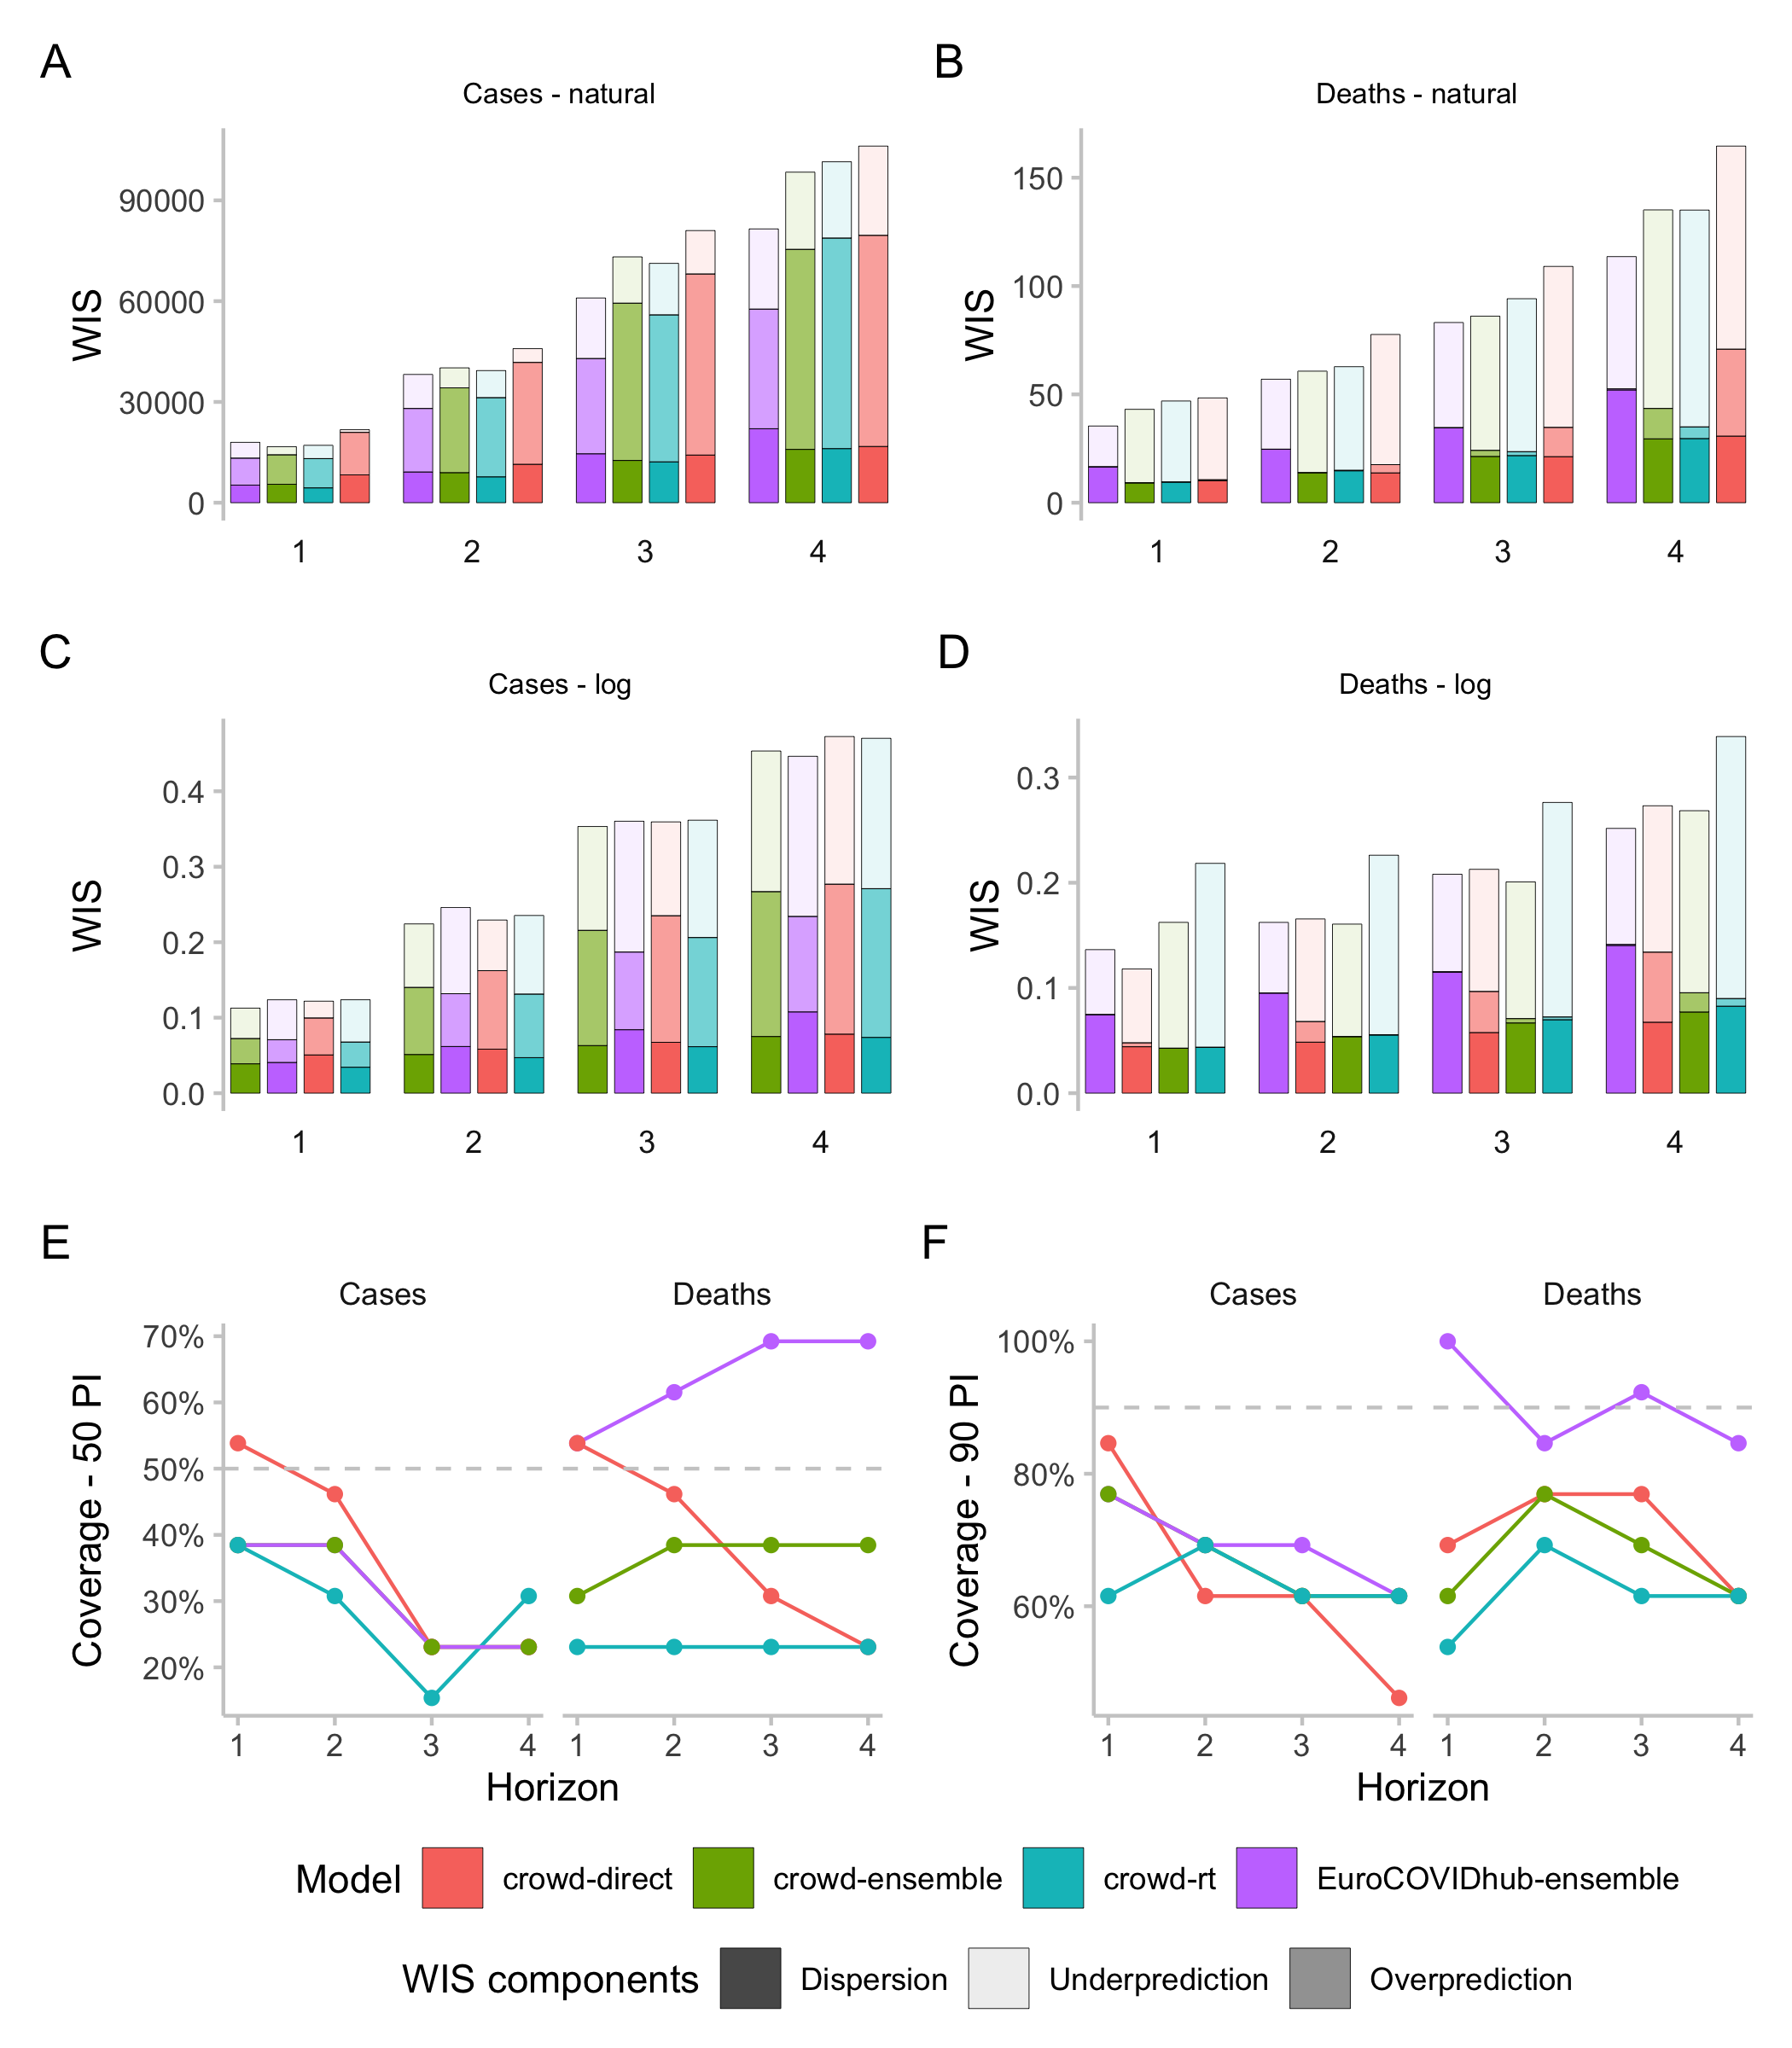
\includegraphics[width=0.99\textwidth]{../output/figures/performance.png}
\caption{\bf{Predictive performance across forecast horizons.} A-D: WIS stratified by forecast horizon for cases and deaths on the natural and log scale. E, F: Empirical coverage of the 50\% and 90\% prediction intervals stratified by forecast horizon and target type.}
\label{fig:performance}
\end{figure*}

\begin{figure*}
\centering
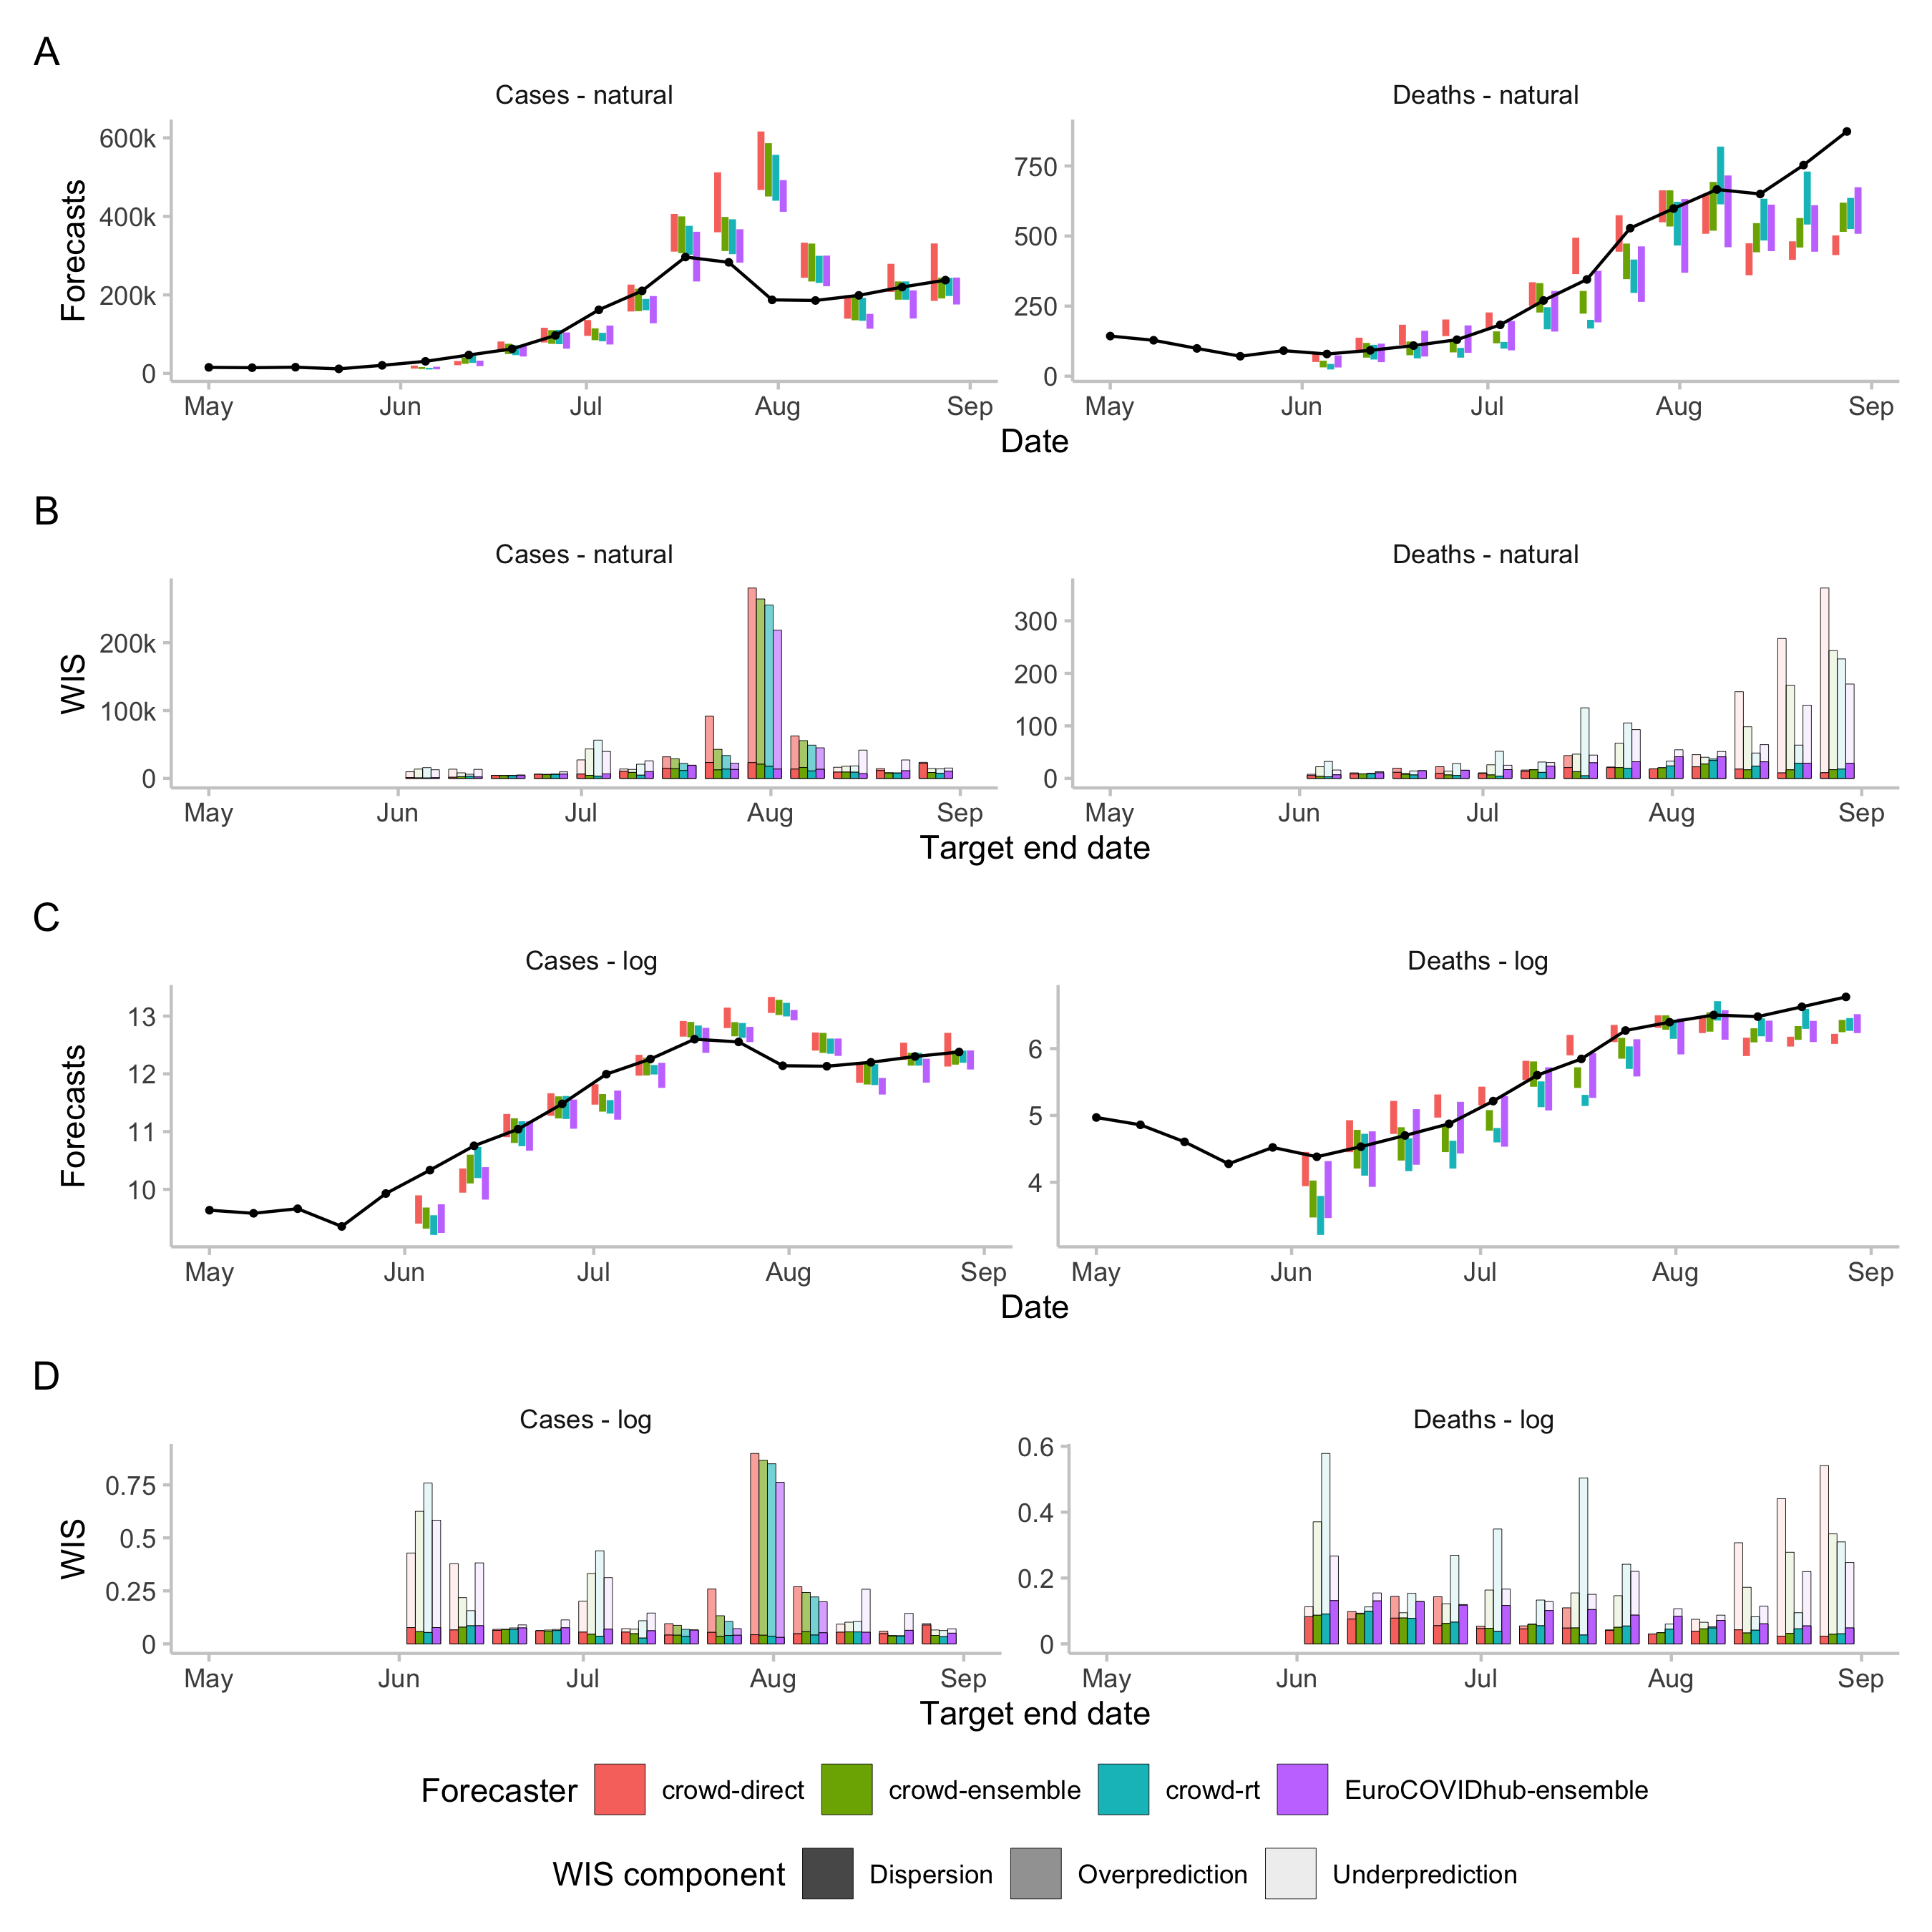
\includegraphics[width=0.99\textwidth]{../output/figures/scores-and-forecasts.png}
\caption{\bf{Forecasts and corresponding WIS for 2-week ahead forecasts of cases and deaths from COVID-19 in the UK.} A: 50\% prediction intervals (coloured bars) and observed values (black line and points) for cases and deaths on the natural scale. B: Corresponding WIS values, decomposed into dispersion, overprediction and underprediction. C: 50\% prediction intervals on the log scale, i.e. after applying the natural logarithm to all forecasts and observations. D: Corresponding WIS on the log scale, i.e. the WIS applied to the log-transformed forecasts and observations.} 
\label{fig:forecasts-scores} 
\end{figure*}

\subsection*{Case forecasts}

All forecasting approaches exhibited underdispersion when predicting cases, meaning that forecasts on average were too narrow and not uncertain enough. Empirical coverage was below nominal coverage for all forecasts and forecast horizons. 
For 50\% prediction intervals, empirical coverage was worst for the direct crowd forecasts (0.31), best for the $R_t$ forecasts (0.46) and in between for the Hub ensemble and the crowd ensemble (both 0.38, see Table \ref{tab:scores}). For 90\% prediction intervals, coverage was worst for the $R_t$ forecasts (0.62) and slightly better for the other approaches (all 0.69). Coverage for all forecasts deteriorated further with increasing forecast horizon (see Figure \ref{fig:performance}). 
%This underdisperion for case forecasts is in line with what was observed previously for case forecasts \citep{bosseComparingHumanModelbased2022, sherrattPredictivePerformanceMultimodel2022a}, all forecasting approaches exhibited underdispersion, 

In terms of WIS on the log scale, all human forecasting approaches outperformed the Forecast Hub ensemble for two week ahead forecasts of cases (see Figure \ref{fig:performance}). WIS values relative to the Hub ensemble (=1) were 0.91 for the combined crowd ensemble, 0.96 for the direct crowd forecasts and 0.93 for the $R_t$ forecasts (see Table \ref{tab:scores}). 
In terms of WIS on the natural scale, however, the Hub ensemble was ahead of all human forecasting approaches. Relative WIS values on the natural scale for two week ahead forecasts were 1.05 for the combined crowd ensemble, 1.03 for the direct crowd forecasts and 1.2 for the $R_t$ forecasts. 

Performance of the Hub ensemble relative to the human forecasting approaches improved with increasing forecast horizon (see Figure \ref{fig:performance}). For a four-week-ahead forecast horizon, the Hub ensemble outperformed all other approaches both on the log scale (rel. WIS values the human forecasts of 1.02, 1.05, 1.06) and on the natural scale (rel. WIS values of 1.21, 1.25, 1.3) (see Table \ref{tab:scores-4}). 

In terms of relative model ranks for two week ahead forecasts, the Hub ensemble and the $R_t$ show a higher variance than the combined crowd ensemble and the direct forecasts (See Figure \ref{fig:performance-ranks}). Both the Hub ensemble and the $R_t$ forecast are most often in the first place, but also most often in the last place. The direct forecasts places relatively equally in places 1-4. The crowd ensemble never places fourth, but also has the lowest number of first places. Model ranks only change marginally when switching between the log and the natural scale. 

When comparing WIS values on the log scale with those on the natural scale, scores were more equally distributed across the study period on the log scale and more weight was given to forecasts in June and July which underpredicted the extent to which case number would rise (see Figure \ref{fig:forecasts-scores}).
On the natural scale, the WIS as a measure of the absolute distance between forecast and observation increased or decreased with the magnitude of the forecast target \cite{bosseTransformationForecastsEvaluating2023, bracherEvaluatingEpidemicForecasts2021}. Average scores were therefore dominated by performance around the peak when cases were highest, in particular by forecasts made on the 19th of July for the 31st of July (see Figure \ref{fig:forecasts-scores}). Switching between scores on the log and on the natural scale had the strongest effect on the $R_t$ forecasts, which had a relative WIS value of 0.96 on the log scale and 1.2 on the natural scale. The $R_t$ forecasts tended to be higher than both the direct forecasts and the Forecast Hub ensemble, especially around the peak and were most severely penalised for overprediction (see Figure \ref{fig:performance}A). On the log scale, underprediction played a larger role, favouring the $R_t$ forecasts (see Figure \ref{fig:performance}C). 

\begin{figure*}
\centering
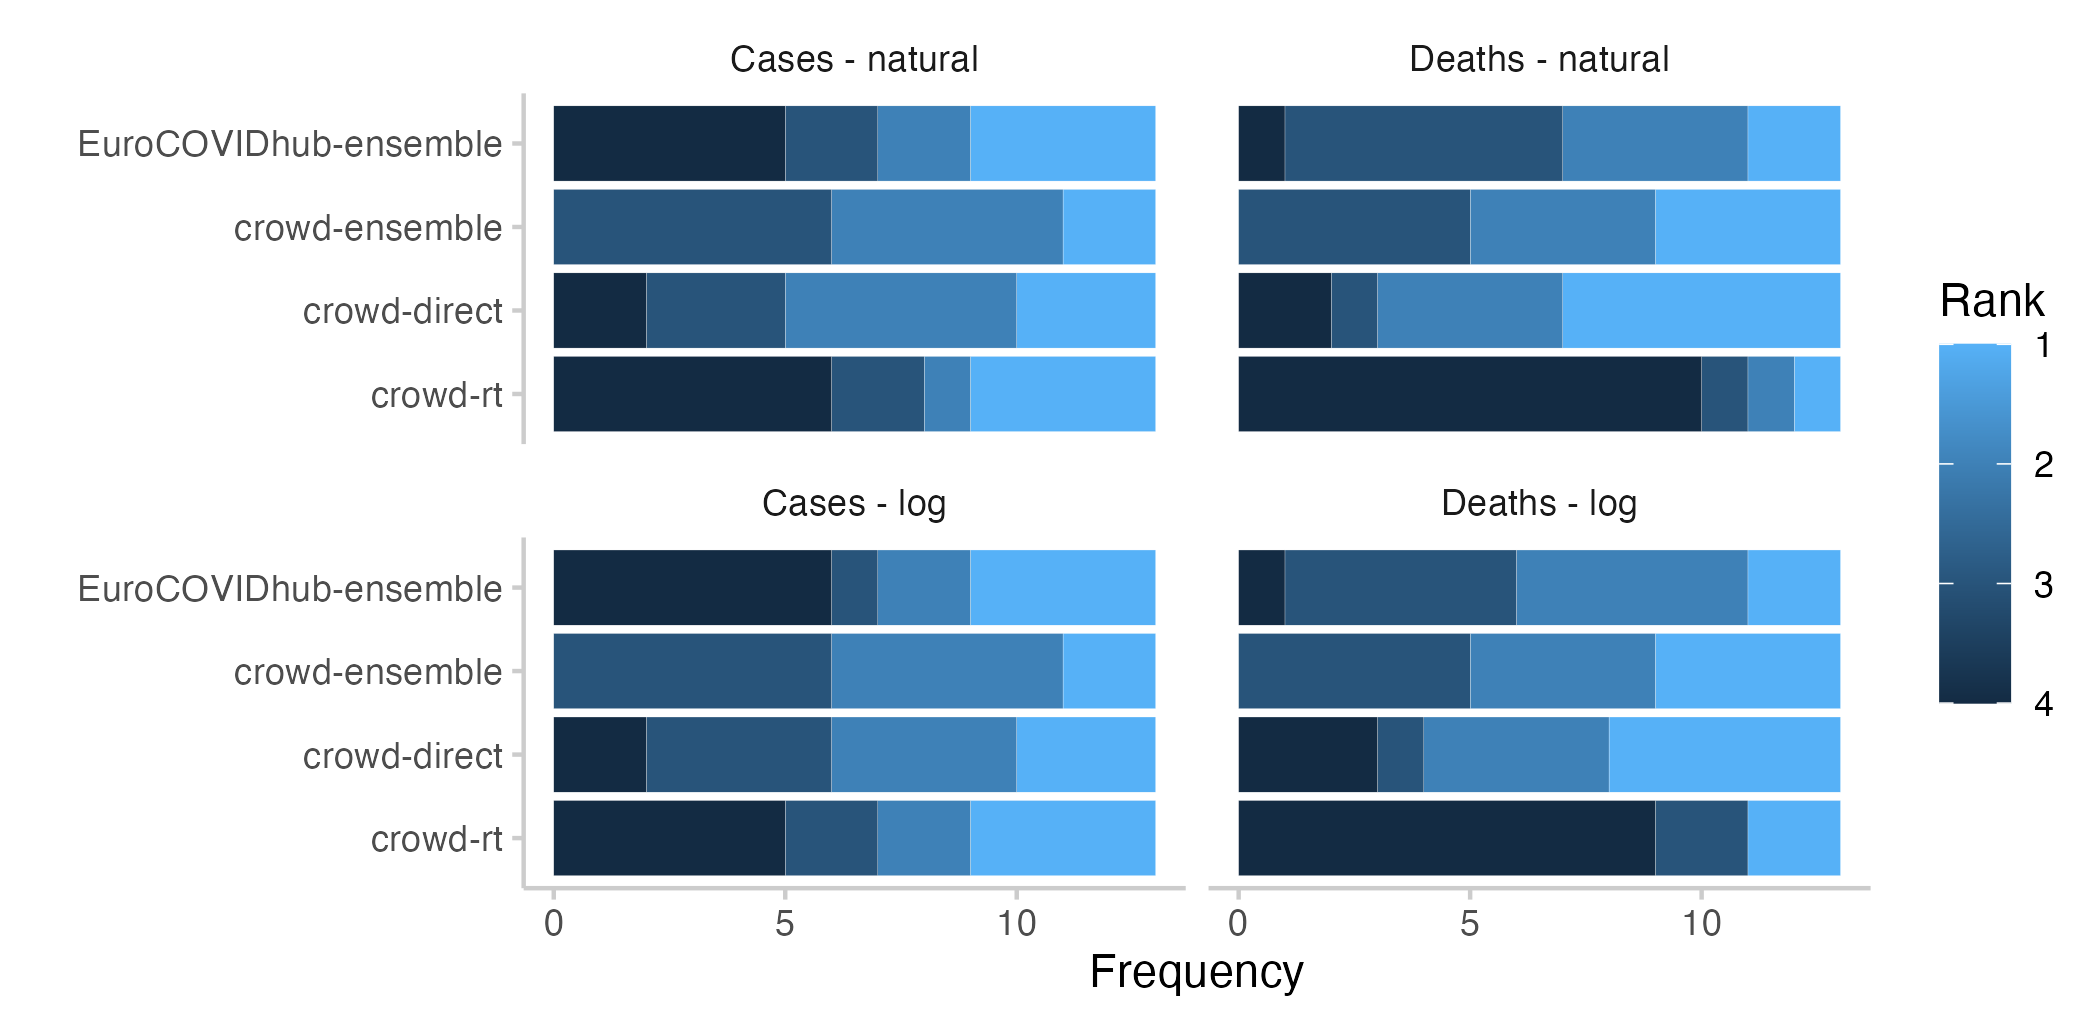
\includegraphics[width=0.99\textwidth]{../output/figures/performance-ranks.png}
\caption{\bf{Performance ranks}....}
\label{fig:performance-ranks}
\end{figure*}

\begin{figure*}
\centering
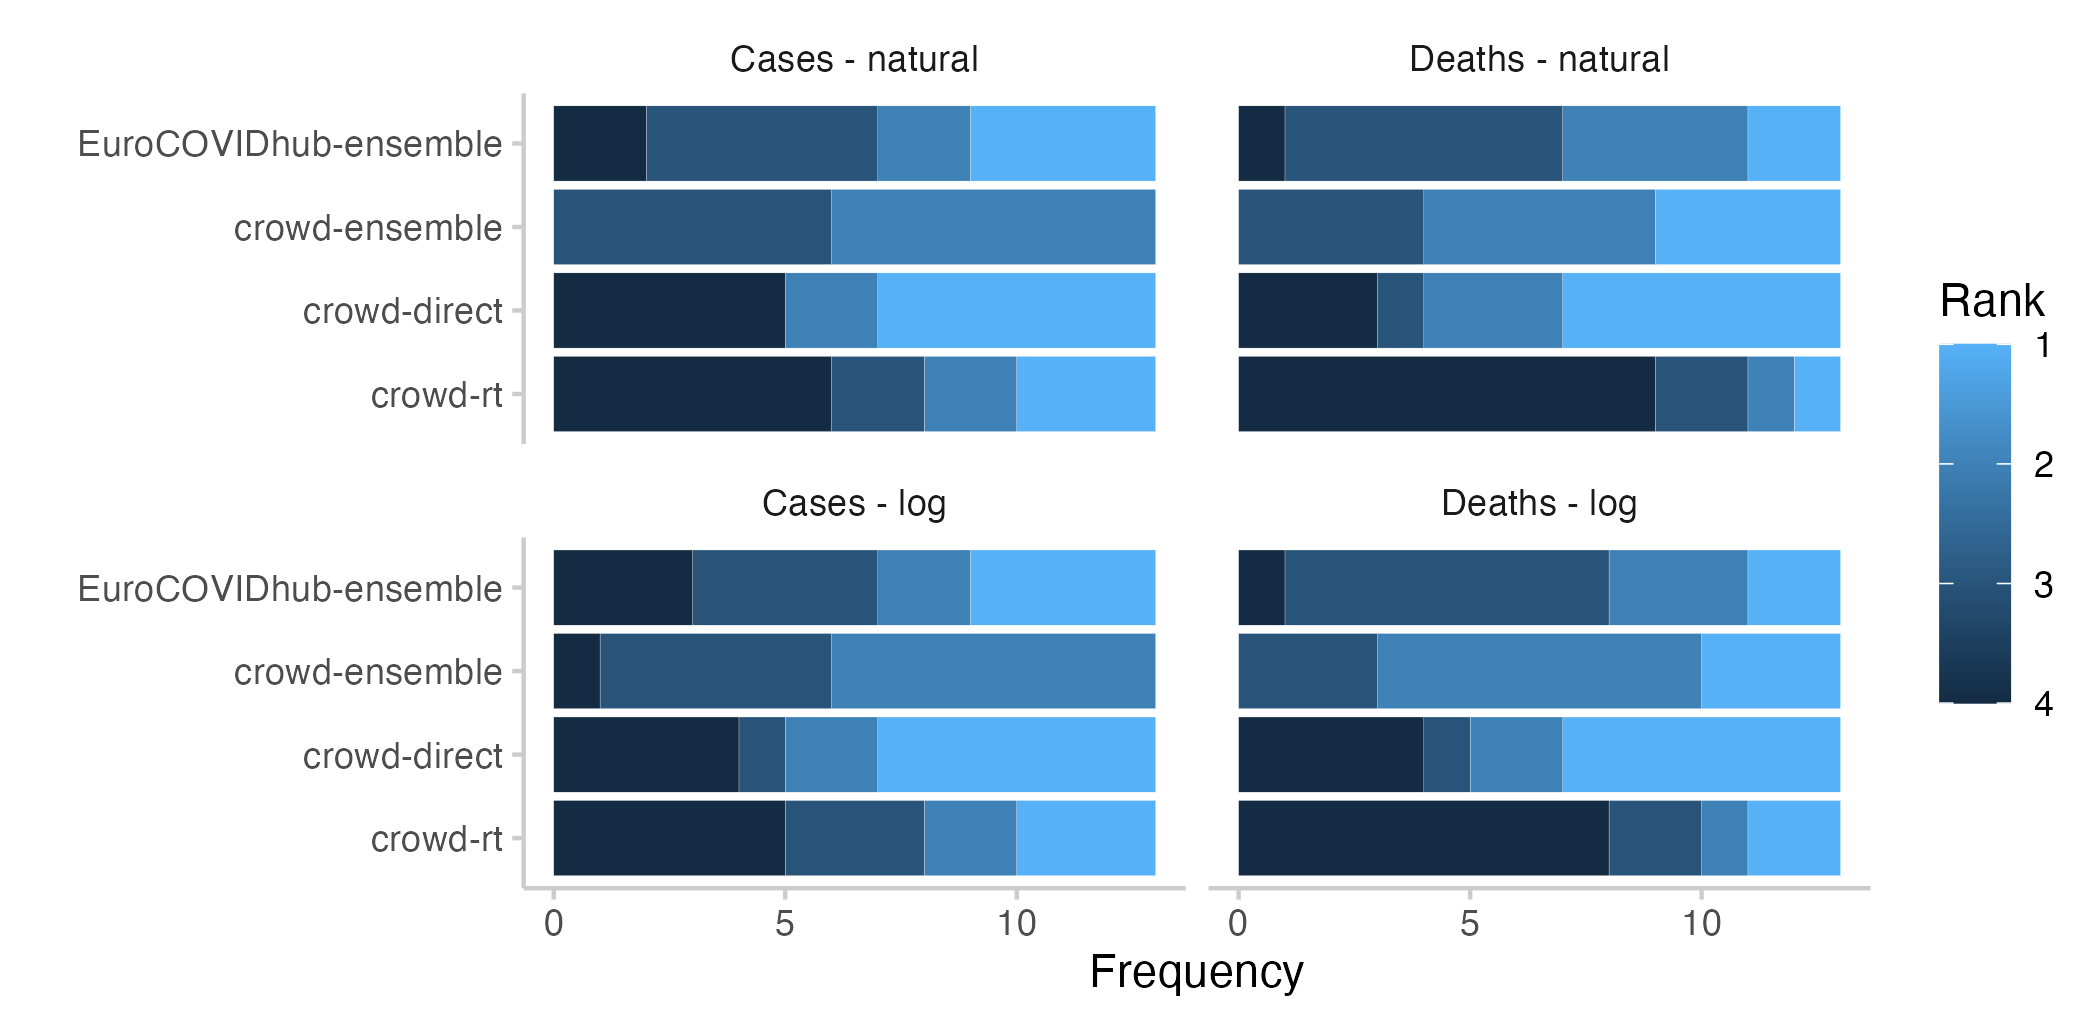
\includegraphics[width=0.99\textwidth]{../output/figures/performance-ranks-4.png}
\caption{\bf{Performance ranks}....}
\label{fig:performance-ranks-4}
\end{figure*}


\subsection*{Death forecasts} 

All forecasting approaches except the $R_t$ forecasts showed higher empirical coverage for deaths than for cases (see Figure \ref{fig:performance}). For 50\% prediction intervals, the Hub ensemble exceeded the nominal coverage noticeably (0.77) (see Table \ref{tab:scores}). $R_t$ forecasts failed to get close to nominal coverage (0.15), while the combined crowd ensemble and the direct forecasts had empirical coverage close to nominal coverage (both 0.54). For 90\% prediction intervals, the Hub ensemble again exceeded nominal coverage and covered all observations (1) while the $R_t$ forecasts again failed to get close to nominal coverage (0.46). The crowd ensemble exhibited a some underdispersion (0.77) while the direct forcecasts almost reached nominal coverage for two week ahead forecasts of deaths (0.85). 

In terms of WIS on the log scale for two week ahead predictions of deaths, the combined crowd ensemble (0.07) and the direct crowd forecasts (0.99) were slightly ahead of the Hub ensemble, while the $R_t$ forecasts performed noticeably worse (1.98) (see Figure \ref{fig:performance} and Table \ref{tab:scores}). Interestingly, combining the $R_t$ forecasts and the direct forecasts led to an ensemble that performed better than either of them. 
In terms of WIS on the natural scale, only the direct forecasts (0.89) performed better for two week ahead death predictions than the Hub ensemble, while the combined crowd ensemble performed a bit worse (1.06) and the $R_t$ forecasts again noticeably worse (2.1). 

% Maybe say something about increasing forecast horizons. But the pattern is unclear. 

In terms of relative model ranks for two week ahead death forecasts, the $R_t$ forecasts took the fourth place most often, while the direct forecasts placed first most often (see Figure \ref{fig:performance-ranks)}. Again, the crowd ensemble never placed fourth.  

When comparing scores on the log and on the natural scale, scores on the log scale are again more evenly distributed across the study period. On the natural scale, high scores were concentrated around the end of the study period, were death incidences were highest (see Figure \ref{fig:forecasts-scores}). 

\subsection*{Rt forecasts}

\begin{figure*}
\centering
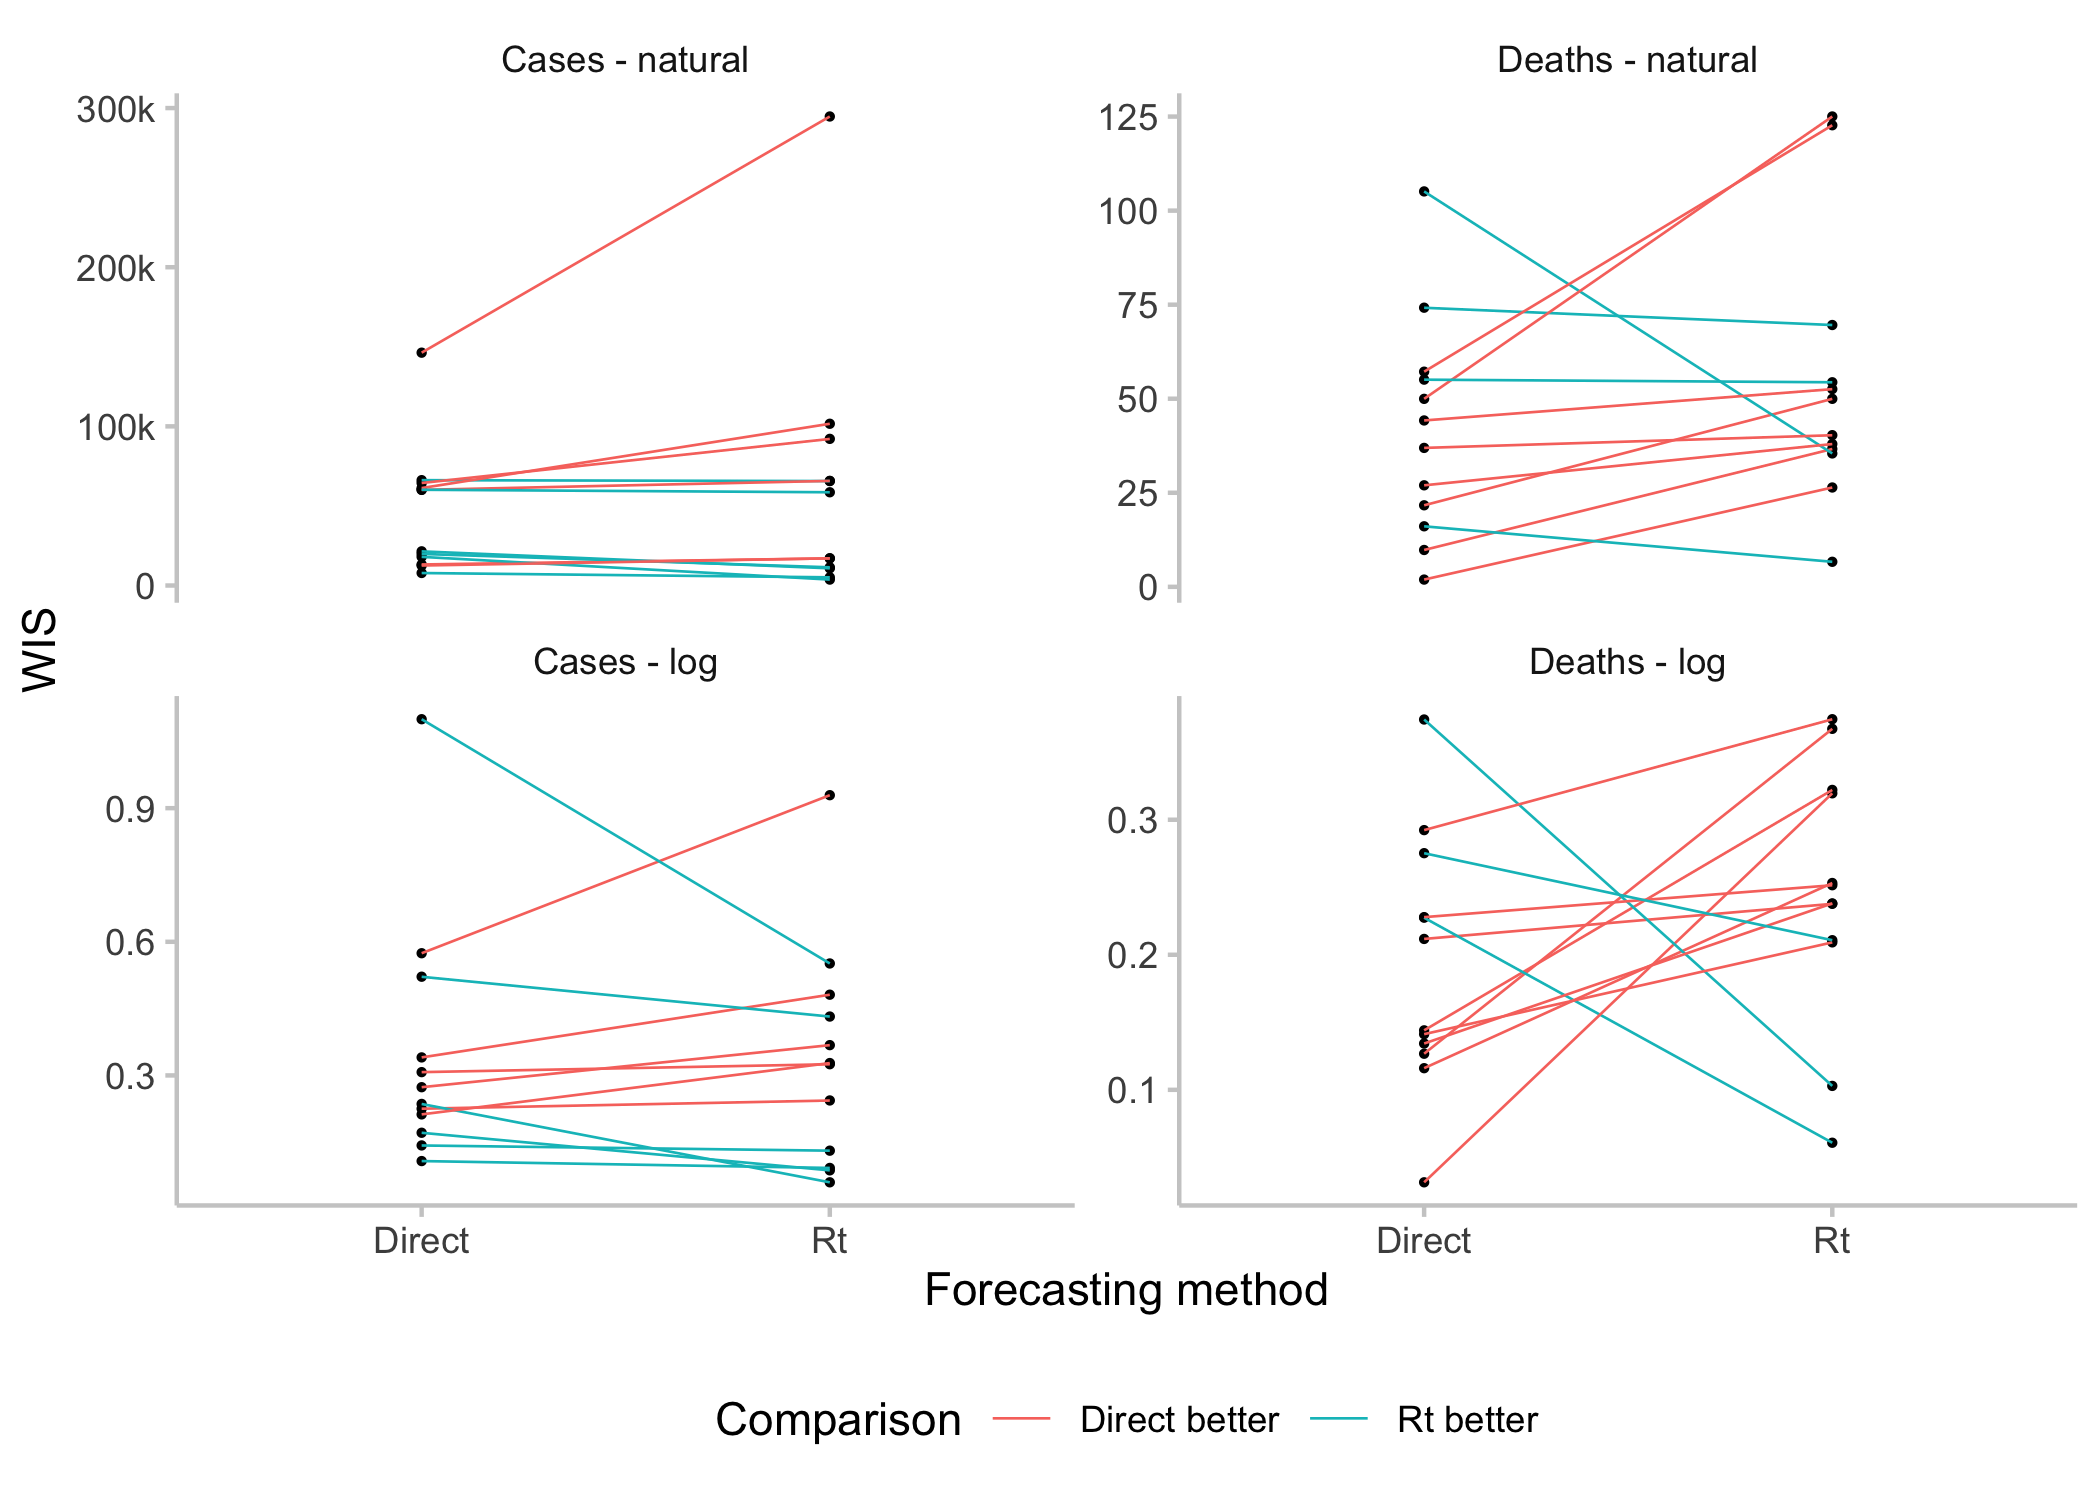
\includegraphics[width=0.99\textwidth]{../output/figures/comparison-direct-rt-individual.png}
\caption{\bf{Comparison of predictive performance of individual forecasters using either the direct forecasting or $R_t$ interface}. Comparisons are based only on those instances where forecasters have submitted a prediction using both interfaces. The absolute level for a given forecaster relative to others is not meaningful as forecasters differ in the amounts of forecasts they have submitted and when.}
\label{fig:comparison-direct-rt-individual}
\end{figure*}

For cases, where participants could observe the case forecast implied by their $R_t$ forecast, predictive performance was similar between corresponding direct and $R_t$ forecasts for most forecasters who had submitted both (see Figure \ref{fig:comparison-direct-rt-individual}). For deaths, where forecasters could not see the incidence forecast implied by their $R_t$ forecast or manually adjust the case fatality rate, performance of the $R_t$ forecasts was significantly worse. From June to the end of July, $R_t$ forecasts overpredicted deaths and were noticeable higher than other forecasts, whereas in August, $R_t$ forecasts underpredicted deaths and were substantially lower than other forecasts (see Figure \ref{fig:forecasts-scores}). In particular, $R_t$ forecasts for deaths were worse than the corresponding direct death forecasts for most forecasters (see Figure \ref{fig:comparison-direct-rt-individual}). Figure \ref{fig:comparison-direct-rt-individual} suggests that changing from the direct forecasting method to $R_t$ forecasting for cases may have improved scores for better forecasters and decreased scores for worse forecasters, although sample sizes are too small to draw definitive conclusions. 



%This suggests that the convolution from latent infections implied by the $R_t$ forecasts to deaths did not capture the relationship between cases and deaths accurately in this instance despite performing well in other settings \citep{meakinComparativeAssessmentMethods2022}. This may be related to changes in the age decomposition of cases and the change in the case fatality ratio (CFR) over the course of the study period due to the rise of the Delta variant starting in May 2021 in the UK. This change was not accounted for in the simple model used and the CFR could not be adjusted by forecasters.

\subsection*{Experts and Non-Experts}

An median ensemble of two week ahead forecasts made only by "experts" or "non-experts" performed worse than the combined crowd example, both for cases and deaths and both on the log scale and on the natural scale (see Table \ref{tab:scores-experts}). 

For cases two week ahead, "experts" achieved better scores than "non-experts" both on the log and on the natural scale. WIS values \textit{relative to the combined crowd ensemble} were 1.08 for "experts" and 1.14 for "non-experts" on the log scale and 1.03 for "experts" and 1.14 for "non-experts" on the natural scale.  

A comparison of "experts" and "non-experts" (self-reported experience in infectious disease modelling or a related field) showed similar performance, both on the natural (WIS two weeks ahead: 43k for experts vs. 43k for non-experts for cases, 41 vs. 46 for deaths) and the log scale (0.24 vs. 0.26 for cases, 0.16 vs. 0.13 for deaths, see Figure \ref{fig:performance-experts}) and Table \ref{tab:scores-expert}. Precise results changed depending on whether or not direct forecasts, $R_t$ forecasts or both were scored. 

% As a direct comparison of individual scores between "experts" and "non-experts" is biased by missing forecasts, 

\section*{Discussion}
% The discussion should include the implications of the article results in view of prior work in this field.

% \paragraph{Summary}

In this paper, we presented a follow-up study to \cite{bosseComparingHumanModelbased2022}, analysing human judgement forecasts of cases of and deaths from COVID-19 in the United Kingdom submitted to the European COVID-19 Forecast Hub between the 24th of May and the 16th of August 2021. Human judgement forecasts were generated using two different forecasting approaches, a) direct forecasts of cases and deaths and b) forecasts of the effective reproduction number $R_t$, which were based on estimates from an open source effective reproduction number estimation model and also relied on this model to generate simulated reported cases and deaths and an extension which estimated a fixed case fatality ratio and a log normal delay between cases and reports. For case numbers, performance of the human judgement forecasts was broadly comparable to the ensemble of all models submitted to the European Forecast Hub, with results changing depending on the forecast horizon and whether or not forecasts were transformed before scoring. The Hub ensemble tended to perform better on longer forecast horizons and when evaluated on the natural scale, while human judgment forecasts tended to perform better for shorter horizons and when evaluated on the log scale. 
%We found that human judgement forecasts of case numbers, regardless of how they were obtained, showed performance broadly comparable to the ensemble of all forecasts submitted to the European Forecast Hub. 
For deaths, performance of direct human forecasts was broadly comparable to that of the Forecast Hub ensemble (with results again changing depending on the forecast horizons and whether or not forecasts were transformed before scoring), while $R_t$ forecasts performed significantly worse. The ensemble that combined $R_t$ and direct forecasts performed only slightly worse than the direct forecasts on the natural scale and was the best performing model on the log scale, in spite of the poor performance of the $R_t$ forecasts.  

%This underdisperion for case forecasts is in line with what was observed previously for case forecasts \citep{bosseComparingHumanModelbased2022, sherrattPredictivePerformanceMultimodel2022a}, all forecasting approaches exhibited underdispersion, 


% \paragraph{Literature context}

In their original study conducted in Germany and Poland, \citet{bosseComparingHumanModelbased2022} humans outperformed an ensemble of computational models when predicting cases, but not when predicting deaths. They hypothesised that computational models might have an advantage over human forecasters when predicting deaths, benefiting from the ability to model the delays and epidemiological relationships between different leading and lagged indicators. \citet{mcandrewChimericForecastingCombining2022} similarly found in their study that humans performed comparably to an ensemble of computational models for cases, but not for predictions of deaths of COVID-19. 
Results in this study did not show the same pattern. We found that in terms of the WIS \textit{on the natural scale}, direct human forecasts were slightly worse than the Forecast Hub ensemble for cases, and slightly better for deaths (although results for greater forecast horizons differed, as did results for the $R_t$ forecasts). Looking at scores \textit{on the log scale}, our study suggests overall comparable performance of the Hub ensemble and the direct human forecasts on both cases and deaths. Relatively good performance of direct human judgement forecasts for death forecasts compared to previous studies may be related to the rise of the Delta variant in the UK starting in the beginning of May. The Delta variant had a higher case fatality ratio (CFR) than previous variants \cite{linDiseaseSeverityClinical2021}. One possible hypothesis for the relatively good performance of human forecasts for deaths compared to previous studies might be that some models submitted to the Forecast Hub may have been more negatively affected by the changes in CFR during the study period than human forecasters. Given the variability in scores across forecast horizons and evaluation methods, result should be interpreted with care. 



% \paragraph{Effort to recruit participants}. 

Just like \citet{bosseComparingHumanModelbased2022} and \citet{farrowHumanJudgmentApproach2017}, this study struggled to retain a large number of participants. Focused public outreach efforts such as creating a dedicated website, announcing an official tournament, providing a public leaderboard, sending weekly emails with details on past performance and weekly announcements on Twitter, did noticeably increase participation compared to the previous study in Germany and Poland. Nevertheless, retaining participants beyond the initial recruitment proved challenging, and most forecasters only submitted a single forecast. \citet{mcandrewChimericForecastingCombining2022} had a higher number of participants, suggesting that making use of existing forecasting platforms, such as Metaculus or Good Judgement Open that provide access to a large existing user base may be helpful in recruiting a larger number of participants though these lack the flexibility and software tooling to run a novel study of this kind in real-time as things stand.

% \paragraph{Expertise}

In our study, an ensemble of only self-reported "experts" did not outperform "non-experts", and even performed worse when looking only at direct forecasts of deaths (but comparably when including $R_t$ forecasts). Past expert forecasts of COVID-19 \cite{recchiaHowWellDid2021} had found predictions from experts to outperform those of non-experts. Our results should be taken with care in light of low sample sizes, and given that expert status was self-reported. Furthermore, we only asked for professional involvement in a field related to infectious disease modelling, not specifically for familiarity with modelling of COVID-19 in the UK, and only offered participants a binary choice. 



% \paragraph{Rt forecasting}

This study explored a novel method of forecasting infectious diseases that combines a human forecast of the estimated effective reproduction number $R_t$ with epidemiological modelling to map the $R_t$ forecast to a forecast of cases and deaths. One appeal of this approach is that the forecaster can directly forecast the generative process. Computational modelling would then take care of dealing with details such as reporting delays, generation intervals, day of the week periodicity, or the relationship between different indicators. This could help reduce cognitive load, and make it easier to synthesise various sources in information into a single forecast, at least for forecasters who have an intuitive understanding of $R_t$. Anecdotally, forecasters familiar to the authors reported high satisfaction with the forecasting experience. In our study, $R_t$ forecasts of cases were comparable to direct forecasts. However, given that forecasters could simulate cases in the app, it is also possible that forecasters were in reality directly forecasting cases. 
$R_t$ forecasts of deaths (which forecasters could not see in the app) were noticeably worse than direct forecasts of deaths. The computational model underlying our $R_t$ forecasts of deaths estimated a constant CFR and delay distribution using the last X weeks of data, therefore updating relatively slowly to new circumstances and not evolving at all over the forecast period. The CFR, however, changed quite quickly during the study period, both due to the rise of the Delta variant \citep{bastIncreasedRiskHospitalisation2021}, as well as changes in the age distribution of cases in Summer 2021, in parts related to the European Football Championship \citep{dehningImpactEuro20202023}. Forecasters had no way of observing the death forecast implied by their $R_t$ forecast and also had no way to adjust the CFR manually, likely impacting forecast accuracy. Giving human forecasters the ability to adjust the CFR and other model parameters would have increased complexity of the interface, but would have solved issues with the assumptions of the underlying model. Alternatively, a more complex model could have been used which allowed for time-varying CFR estimates and forecast these changes over the forecast horizon. Another potential solution would have been to use the human forecasts for cases as an input to the computational model, which could then have estimated deaths as a convolution of cases over a delay distribution. Future work could expose forecasters to different such options with the aim of separating effects of the user interface from ones related to the structure of the underlying computational model.
%The relationship between cases and deaths used to forecast 
%In addition . The gradual change in the CFR was not accounted for in the computational model underying the $R_t$ forecasts, and estimated distributions from past data only slowly updated to new circumstances. One potential solution for this would be to allow humans to adjust the CFR and other model parameters manually as part of their forecast. 

% \paragraph{Susceptibility of results}

Overall, results of our study should be taken with some caution due to a number of important limitations. Firstly, our study was restricted to one location and to a relatively short period of thirteen weeks. Secondly, there are many confounding factors that can influence results. These include for example the fact that different participants made forecasts at different points in time and that subgroups of interest (e.g. "experts", or $R_t$ forecasts) had different numbers of forecasters. In addition, there are many researcher degrees of freedom that influence results, for example how individual forecasts are combined to an ensemble and how forecasts are evaluated. Prizes to the human forecasters, for example were paid out based on the combined WIS on the log scale across all horizons and forecast targets. Had we chosen to instead measure WIS on the natural scale, rankings and payouts would have been different. 


\section*{Conclusions}
% Please state what you think are the main conclusions that can be realistically drawn from the findings in the paper, taking care not to make claims that cannot be supported.

Overall, the results of our study seem broadly consistent with previous studies on human judgement forecasting of COVID-19 and suggest that human crowd ensembles and an ensemble of computational models can show similar performance. One possible interpretation is that a mixed crowd of human forecaster can produce a viable alternative or addition to an ensemble of mathematical models created by experts. Another interpretation is that an ensemble of automated models can produce forecasts over the course of several years that are on par with that of an engaged crowd of human forecasters. All previous studies comparing human judgement forecasts and computational models only ran over short periods of time and the majority of them struggled with recruitment and upkeep. Meanwhile, COVID-19 Forecast Hubs have attracted continuous submissions for almost three years and were able to consistently provide forecasts of comparable quality. 

Our findings don't suggest that humans are necessarily at a general disadvantage compared to computational models at predicting death numbers, but evidence in both directions is limited and this is made particularly complex as our study took place during a period of time when CFR estimates were changing rapidly. Despite evaluations being public, it remains a challenge to properly incentivise contributors to Forecast Hubs to regularly update their forecasting methodology in order to maximise utility, predictive performance, or both. Combining human judgement and epidemiological modelling by mapping $R_t$ forecasts to case and death numbers has not yielded competitive forecasts for deaths in this study. However, we only presented a prototype of a forecasting approach, which, while having appealing properties, proved challenging to implement. Subsequent iterations and improvements could likely achieve better results. More research is required to obtain a better understanding of the role of subject matter expertise in infectious disease forecasting. Our results underline that it is difficult to evaluate forecast performance devoid of context that helps inform what a good or a bad forecast is. Different ways to look at the data let different forecasts appear good or bad. Forecast evaluation therefore either needs to be clearly informed by the needs of forecast consumers to determine what a good forecast is, or it needs a broad array of perspectives to provide a wholistic picture. Furthermore, evaluating forecasts post-hoc leaves the researchers with many degrees of freedom to make decisions that strongly affect which models look good and there is a high risk of allowing for motivated reasoning. More emphasis should be put on measures that prevent this, e.g. by establishing common standards for evaluations, pre-registering studies, and making it a norm to display a variety of metrics. 








\subsection*{Author contributions}
In order to give appropriate credit to each author of an article, the individual
contributions of each author to the manuscript should be detailed in this section. We
recommend using author initials and then stating briefly how they contributed.

\subsection*{Competing interests}
Nikos I. Bosse is a part-time employee of Metaculus, an online prediction platform. 

\subsection*{Grant information}
Please state who funded the work discussed in this article, whether it is your employer,
a grant funder etc. Please do not list funding that you have that is not relevant to this
specific piece of research. For each funder, please state the funder’s name, the grant
number where applicable, and the individual to whom the grant was assigned.

\subsection*{Acknowledgements}
We thank all forecasters for their participation and want to congratulate the three winners of the forecasting challenge: Russel Bradshaw, Sebastian Funk, and Akira Endo. All winners donated their prizes. 



% ================================= References =============================== %
\clearpage

{\small\bibliographystyle{unsrtnat}
\bibliography{software, uk-forecasting-challenge}}

\bigskip
\clearpage

% =================================== Appendix =============================== %

% Make sure that Appendix tables and Figures are separate
% https://tex.stackexchange.com/questions/520193/is-it-possible-to-except-figures-in-the-appendix-from-being-repositioned-by-endf
\processdelayedfloats
\csname efloat@restorefloats\endcsname

\appendix
\section*{Supplementary information}
\renewcommand{\thefigure}{SI.\arabic{figure}}
\setcounter{figure}{0}
\renewcommand{\thetable}{SI.\arabic{table}} \setcounter{table}{0}


\subsection*{Weighted interval score}
\label{sec:wis}

The weighted interval score (smaller values are better) is a proper scoring rule for quantile forecasts. It converges to the continuous ranked probability score (which itself is a generalisation of the absolute error to probabilistic forecasts) for an increasing number of intervals. The score can be decomposed into a dispersion (uncertainty) component and penalties for over- and underprediction. For a single interval, the score is computed as 
  $$IS_\alpha(F,y) = (u-l) + \frac{2}{\alpha} \cdot (l-y) \cdot 1(y \leq l) + \frac{2}{\alpha} \cdot (y-u) \cdot 1(y \geq u), $$ 
  where $1()$ is the indicator function, $y$ is the true value, and $l$ and $u$ are the $\frac{\alpha}{2}$ and $1 - \frac{\alpha}{2}$ quantiles of the predictive distribution $F$, i.e. the lower and upper bound of a single prediction interval. For a set of $K$ prediction intervals and the median $m$, the score is computed as a weighted sum, 
  $$WIS = \frac{1}{K + 0.5} \cdot \left( w_0 \cdot |y - m| + \sum_{k = 1}^{K} w_k \cdot IS_{\alpha}(F, y) \right), $$
  where $w_k$ is a weight for every interval. Usually, $w_k = \frac{\alpha_k}{2}$ and $w_0 = 0.5$. 

\input SI/epinow2.tex

%table 4 weeks


\begin{table*}[!h]

\caption{Performance for two-week-ahead forecasts of experts and non-experts. Values have been cut to three significant digits and rounded. \label{tab:scores-experts}}
\centering
\resizebox{\linewidth}{!}{
\begin{tabular}[t]{llccccllcc}
\toprule
\multicolumn{2}{c}{ } & \multicolumn{3}{c}{WIS - natural} & \multicolumn{3}{c}{WIS - log scale} & \multicolumn{2}{c}{ } \\
\cmidrule(l{3pt}r{3pt}){3-5} \cmidrule(l{3pt}r{3pt}){6-8}
Model & Target & abs. & rel. & sd & abs. & rel. & sd & Coverage 50\% & Coverage 90\%\\
\midrule
EuroCOVIDhub-ensemble & Cases & 38.2k & 1 & 55.6k & 0.25 & 1 & 0.22 & 0.38 & 0.69\\
 & Cases & 42.7k & 1.12 & 74.9k & 0.24 & 0.98 & 0.28 & 0.46 & 0.77\\
 & Cases & 43.1k & 1.13 & 67k & 0.26 & 1.04 & 0.25 & 0.31 & 0.54\\
EuroCOVIDhub-ensemble & Deaths & 37.9 & 1 & 26.9 & 0.13 & 1 & 0.04 & 0.77 & 1\\
\addlinespace
 & Deaths & 41.2 & 1.09 & 41.8 & 0.16 & 1.25 & 0.15 & 0.54 & 0.77\\
 & Deaths & 45.9 & 1.21 & 56.8 & 0.13 & 1.03 & 0.08 & 0.46 & 0.77\\
\bottomrule
\end{tabular}}
\end{table*}

\begin{table*}[!h]

\caption{Performance for four-week-ahead forecasts of experts and non-experts. Values have been cut to three significant digits and rounded. \label{tab:scores-experts-4}}
\centering
\resizebox{\linewidth}{!}{
\begin{tabular}[t]{llccccllcc}
\toprule
\multicolumn{2}{c}{ } & \multicolumn{3}{c}{WIS - natural} & \multicolumn{3}{c}{WIS - log scale} & \multicolumn{2}{c}{ } \\
\cmidrule(l{3pt}r{3pt}){3-5} \cmidrule(l{3pt}r{3pt}){6-8}
Model & Target & abs. & rel. & sd & abs. & rel. & sd & Coverage 50\% & Coverage 90\%\\
\midrule
EuroCOVIDhub-ensemble & Cases & 38.2k & 1 & 55.6k & 0.25 & 1 & 0.22 & 0.38 & 0.69\\
Expert & Cases & 42.7k & 1.12 & 74.9k & 0.24 & 0.98 & 0.28 & 0.46 & 0.77\\
Non-Expert & Cases & 43.1k & 1.13 & 67k & 0.26 & 1.04 & 0.25 & 0.31 & 0.54\\
\addlinespace
EuroCOVIDhub-ensemble & Deaths & 37.9 & 1 & 26.9 & 0.13 & 1 & 0.04 & 0.77 & 1\\
Expert & Deaths & 41.2 & 1.09 & 41.8 & 0.16 & 1.25 & 0.15 & 0.54 & 0.77\\
Non-Expert & Deaths & 45.9 & 1.21 & 56.8 & 0.13 & 1.03 & 0.08 & 0.46 & 0.77\\
\bottomrule
\end{tabular}}
\end{table*}

\begin{figure*}
\centering
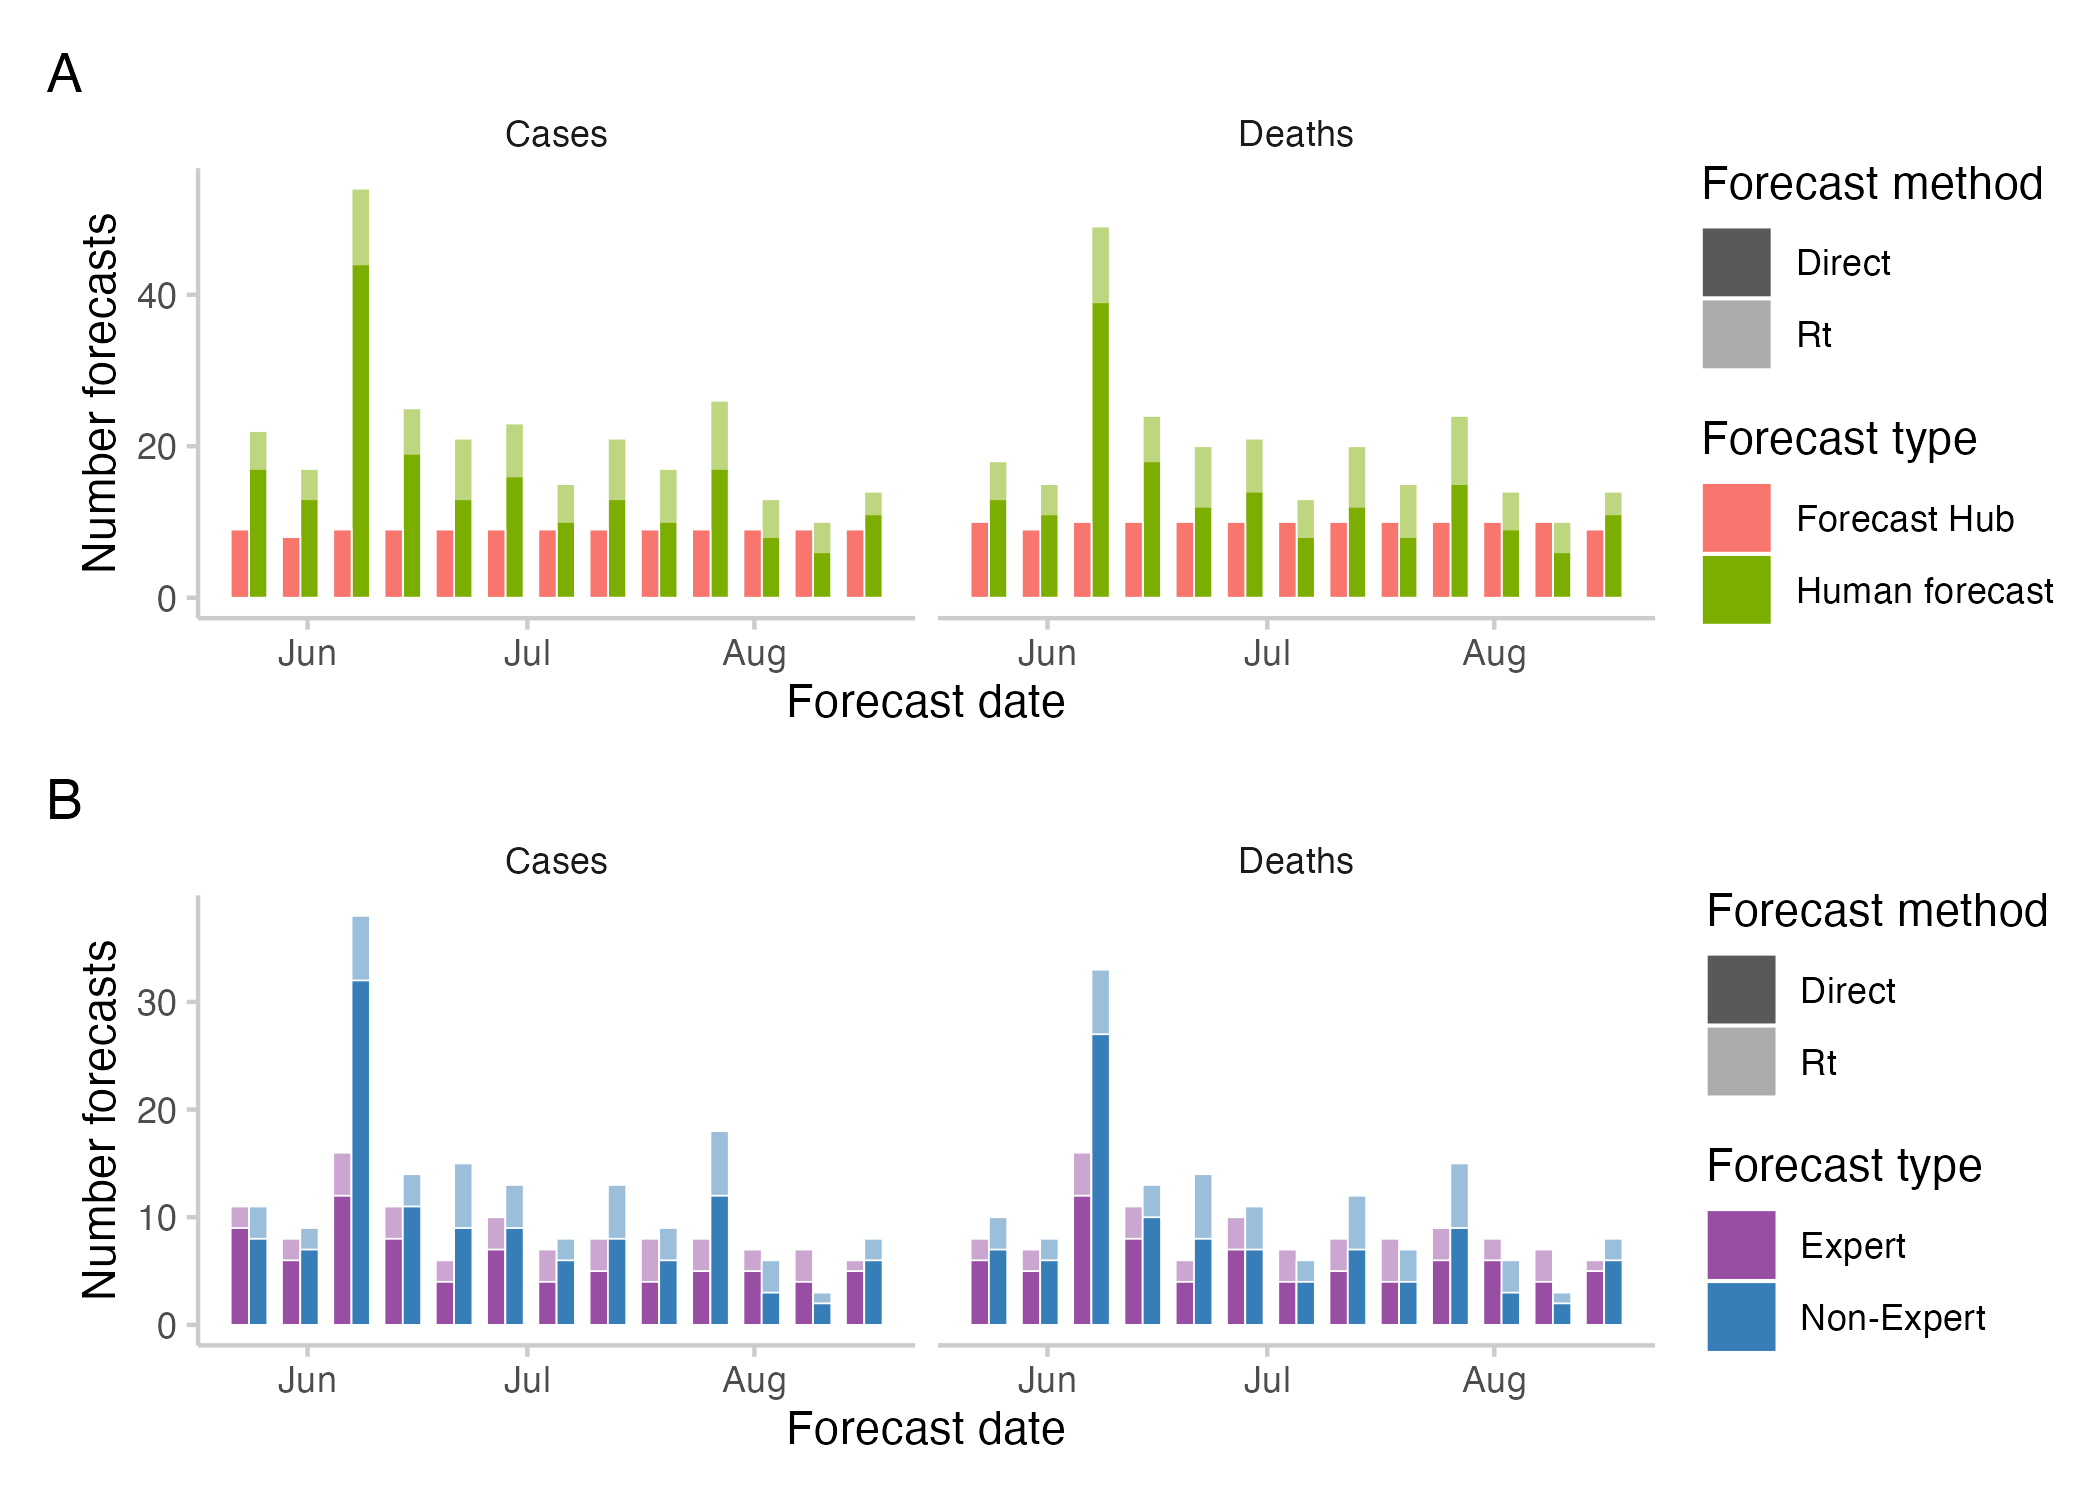
\includegraphics[width=0.99\textwidth]{../output/figures/num-forecasters.png}
\caption{\bf{Number of forecasts across the study period.}}
\label{fig:num-forecasters}
\end{figure*}


\begin{figure*}
\centering
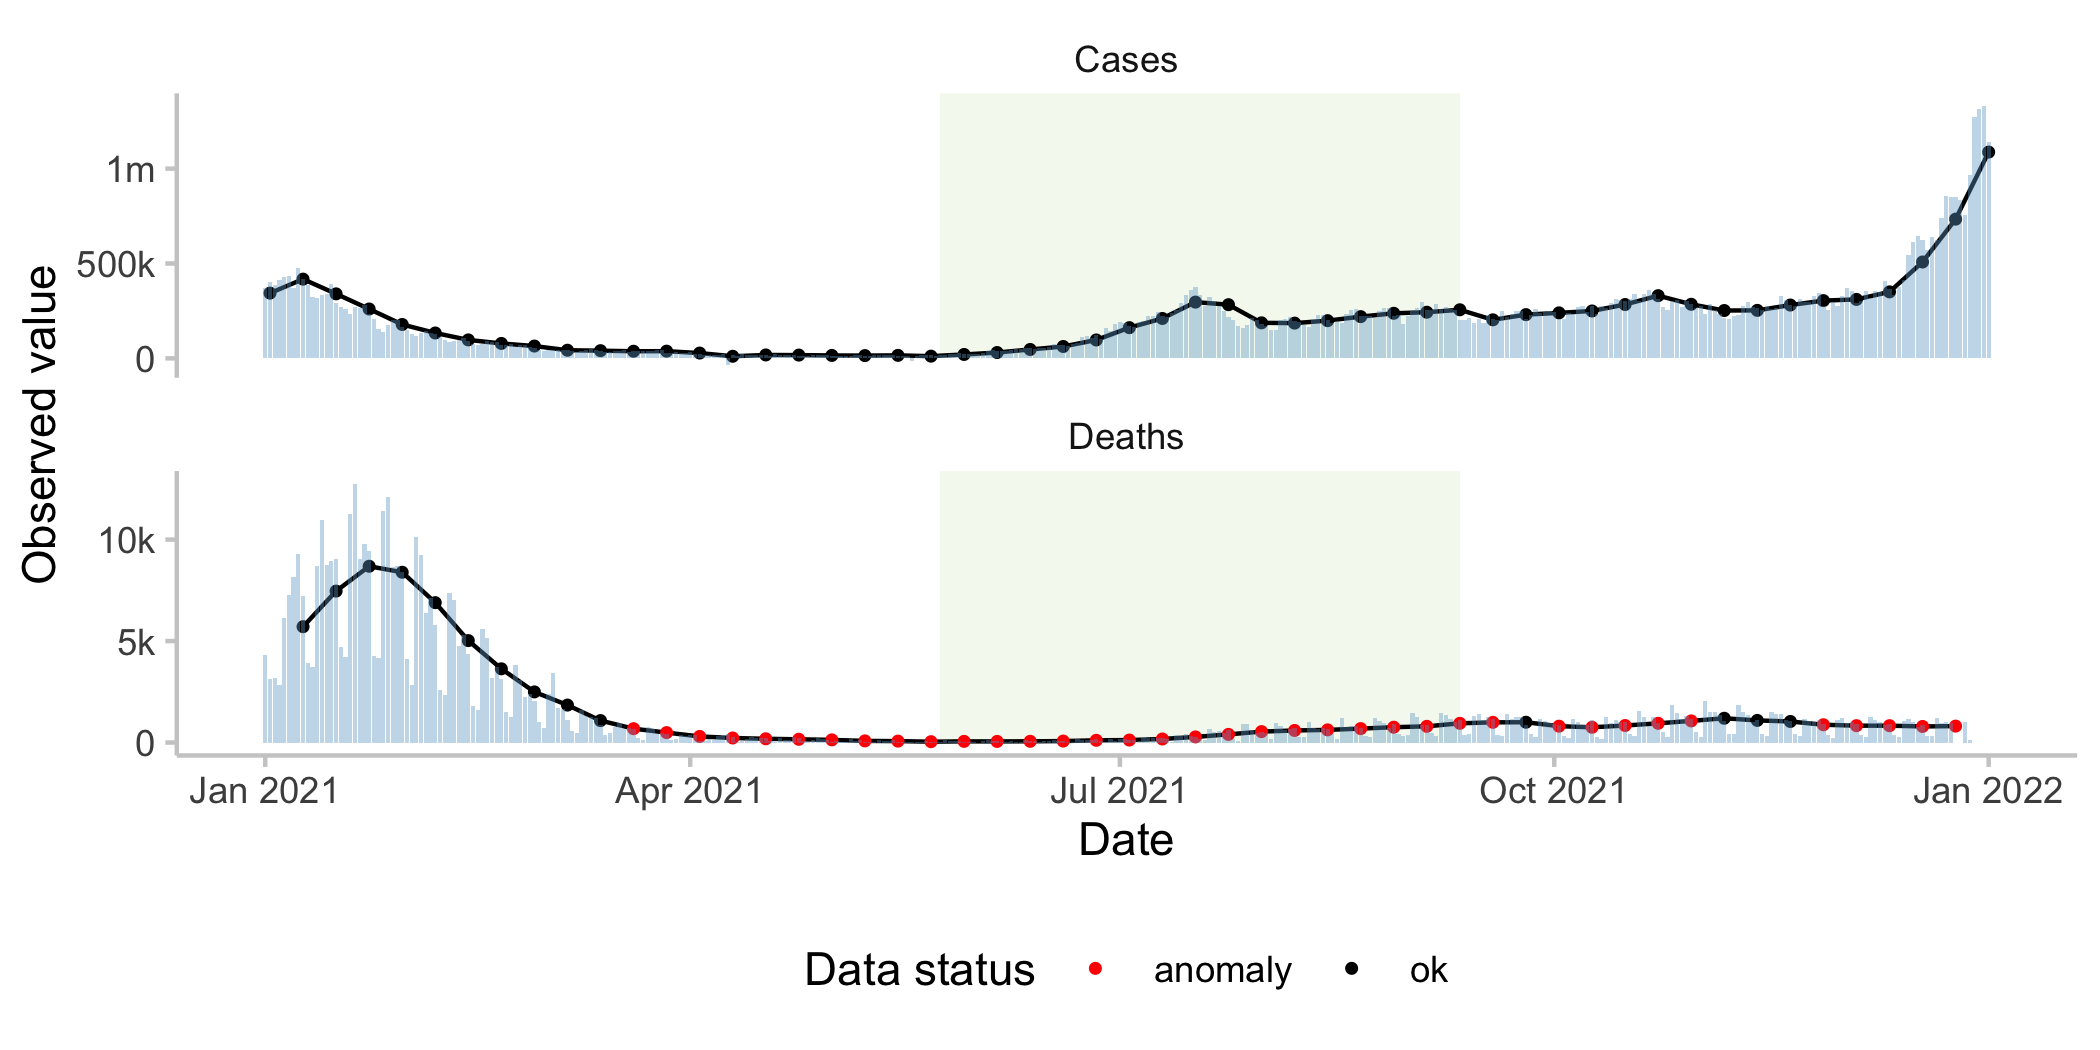
\includegraphics[width=0.99\textwidth]{../output/figures/plot-data.png}
\caption{\bf{Observed cases and deaths of COVID-19 in the UK}. A: Observed daily (bars) and weekly (black lines and points) numbers of cases and deaths as available through the European Forecast Hub when the study concluded in 2021. Daily numbers were multiplied by seven in order to appear on the same scale as weekly numbers. Red dots represent days for which the original data and the revised data disagreed by more than five percent. B: Revised data available as of February 14 2023. In August, Johns Hopkins University that provided the data switched the data stream for their death forecasts to reflect the number of death certificates that mentioned COVID-19 rather than the number of people who died within 28 days of a positive test. C: Difference between the original and revised weekly death numbers.}
\label{fig:plot-data}
\end{figure*}


\begin{figure*}
\centering
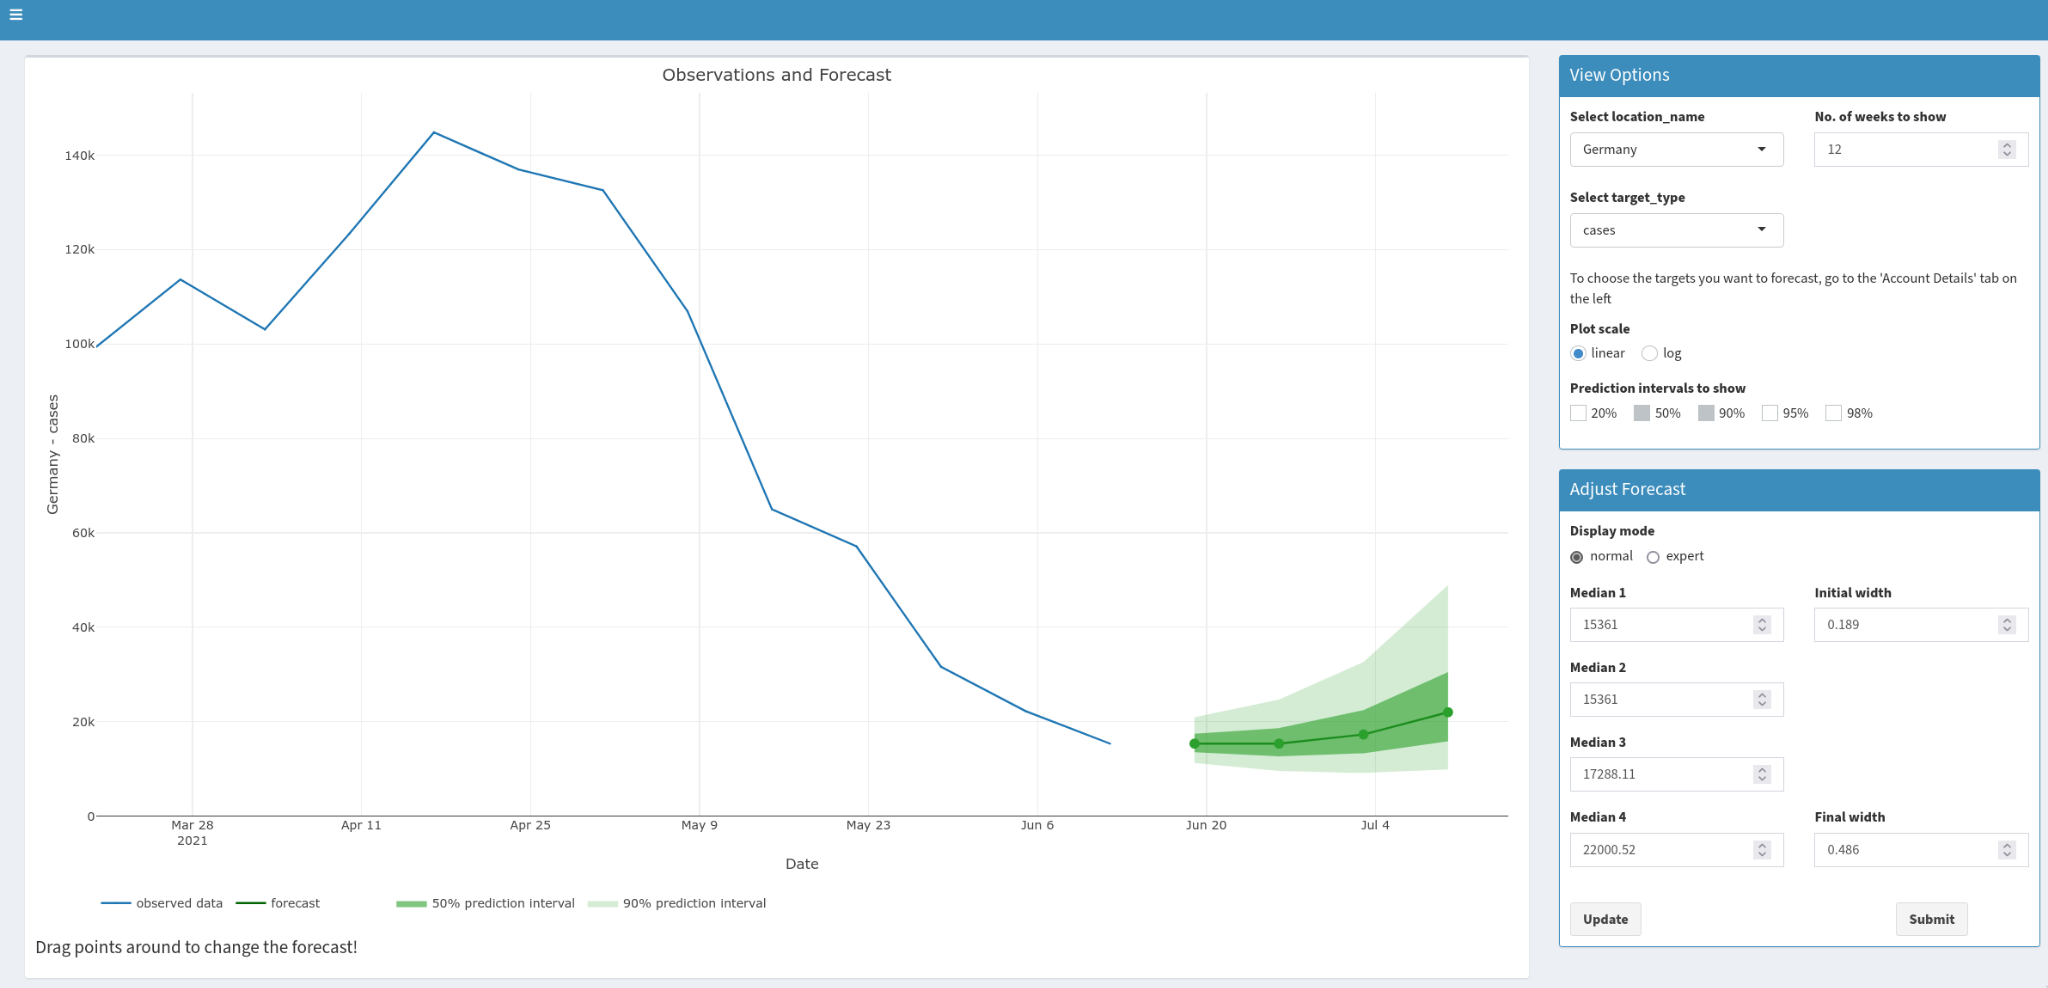
\includegraphics[width=0.99\textwidth]{../output/figures/screenshot-crowd-classical.png}
\caption{\bf{Screenshot of the direct forecasting interface.}}
\label{fig:screenshot-classical}
\end{figure*}


\begin{figure*}
\centering
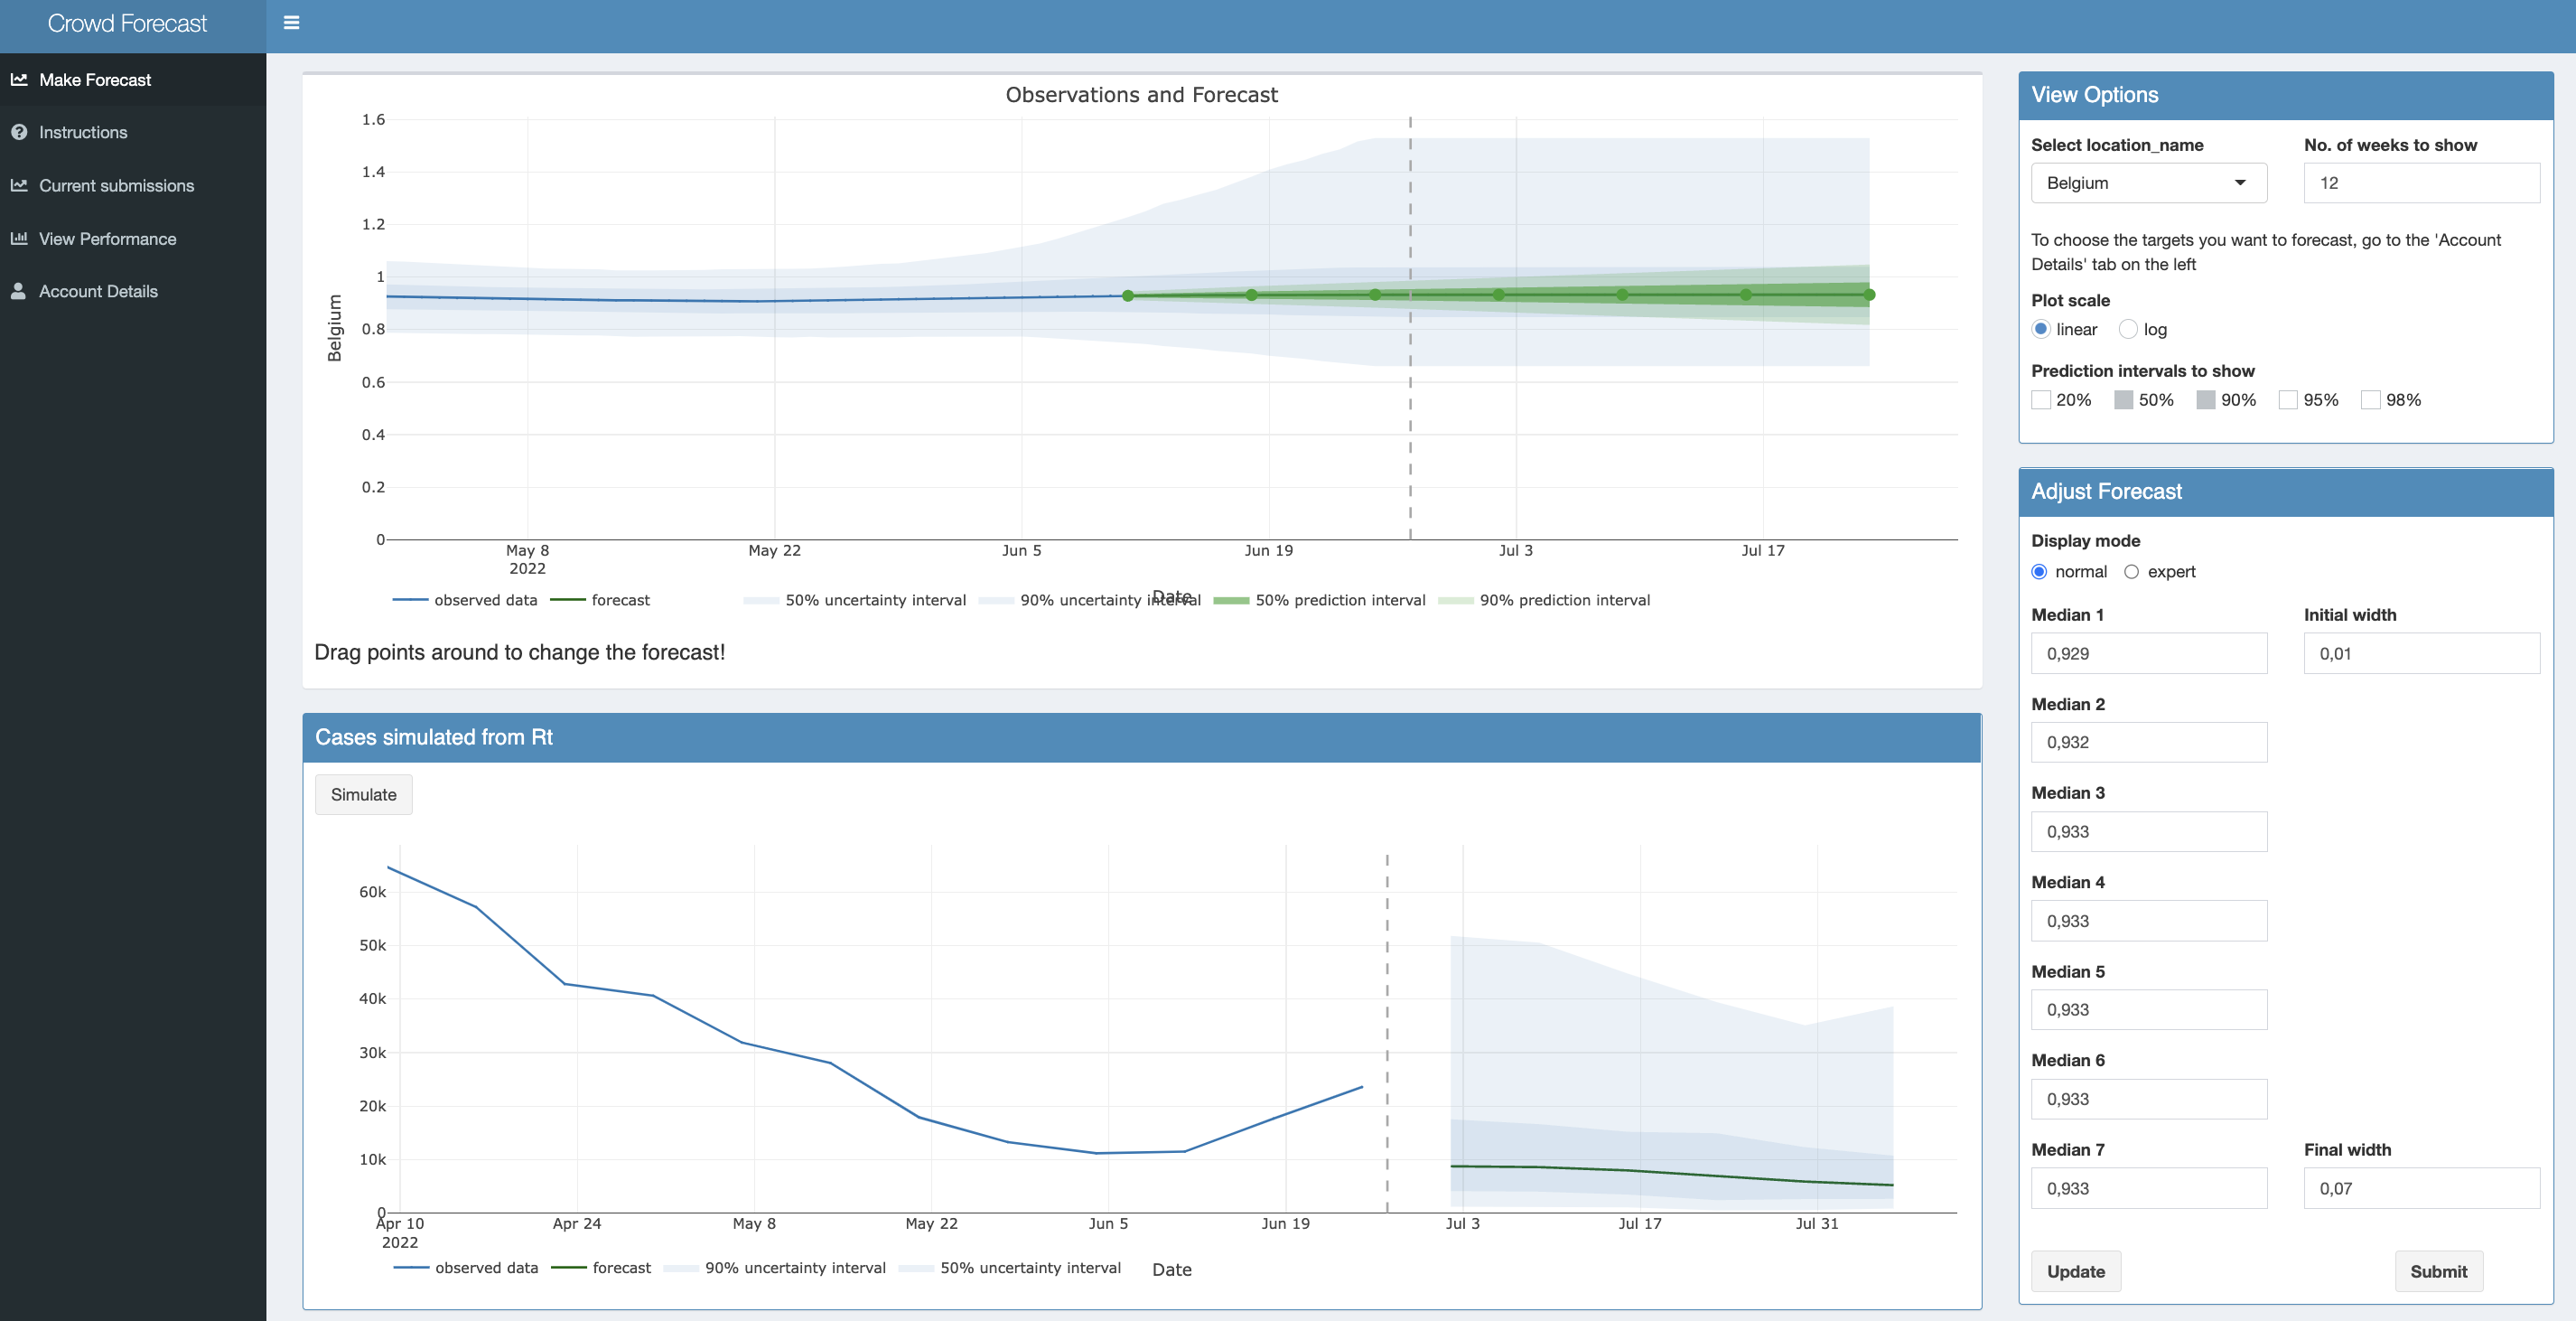
\includegraphics[width=0.99\textwidth]{../output/figures/screenshot-crowd-rt-app.png}
\caption{\bf{Screenshot of the $R_t$ forecasting interface.}}
\label{fig:screenshot-rt}
\end{figure*}

\begin{figure*}
\centering
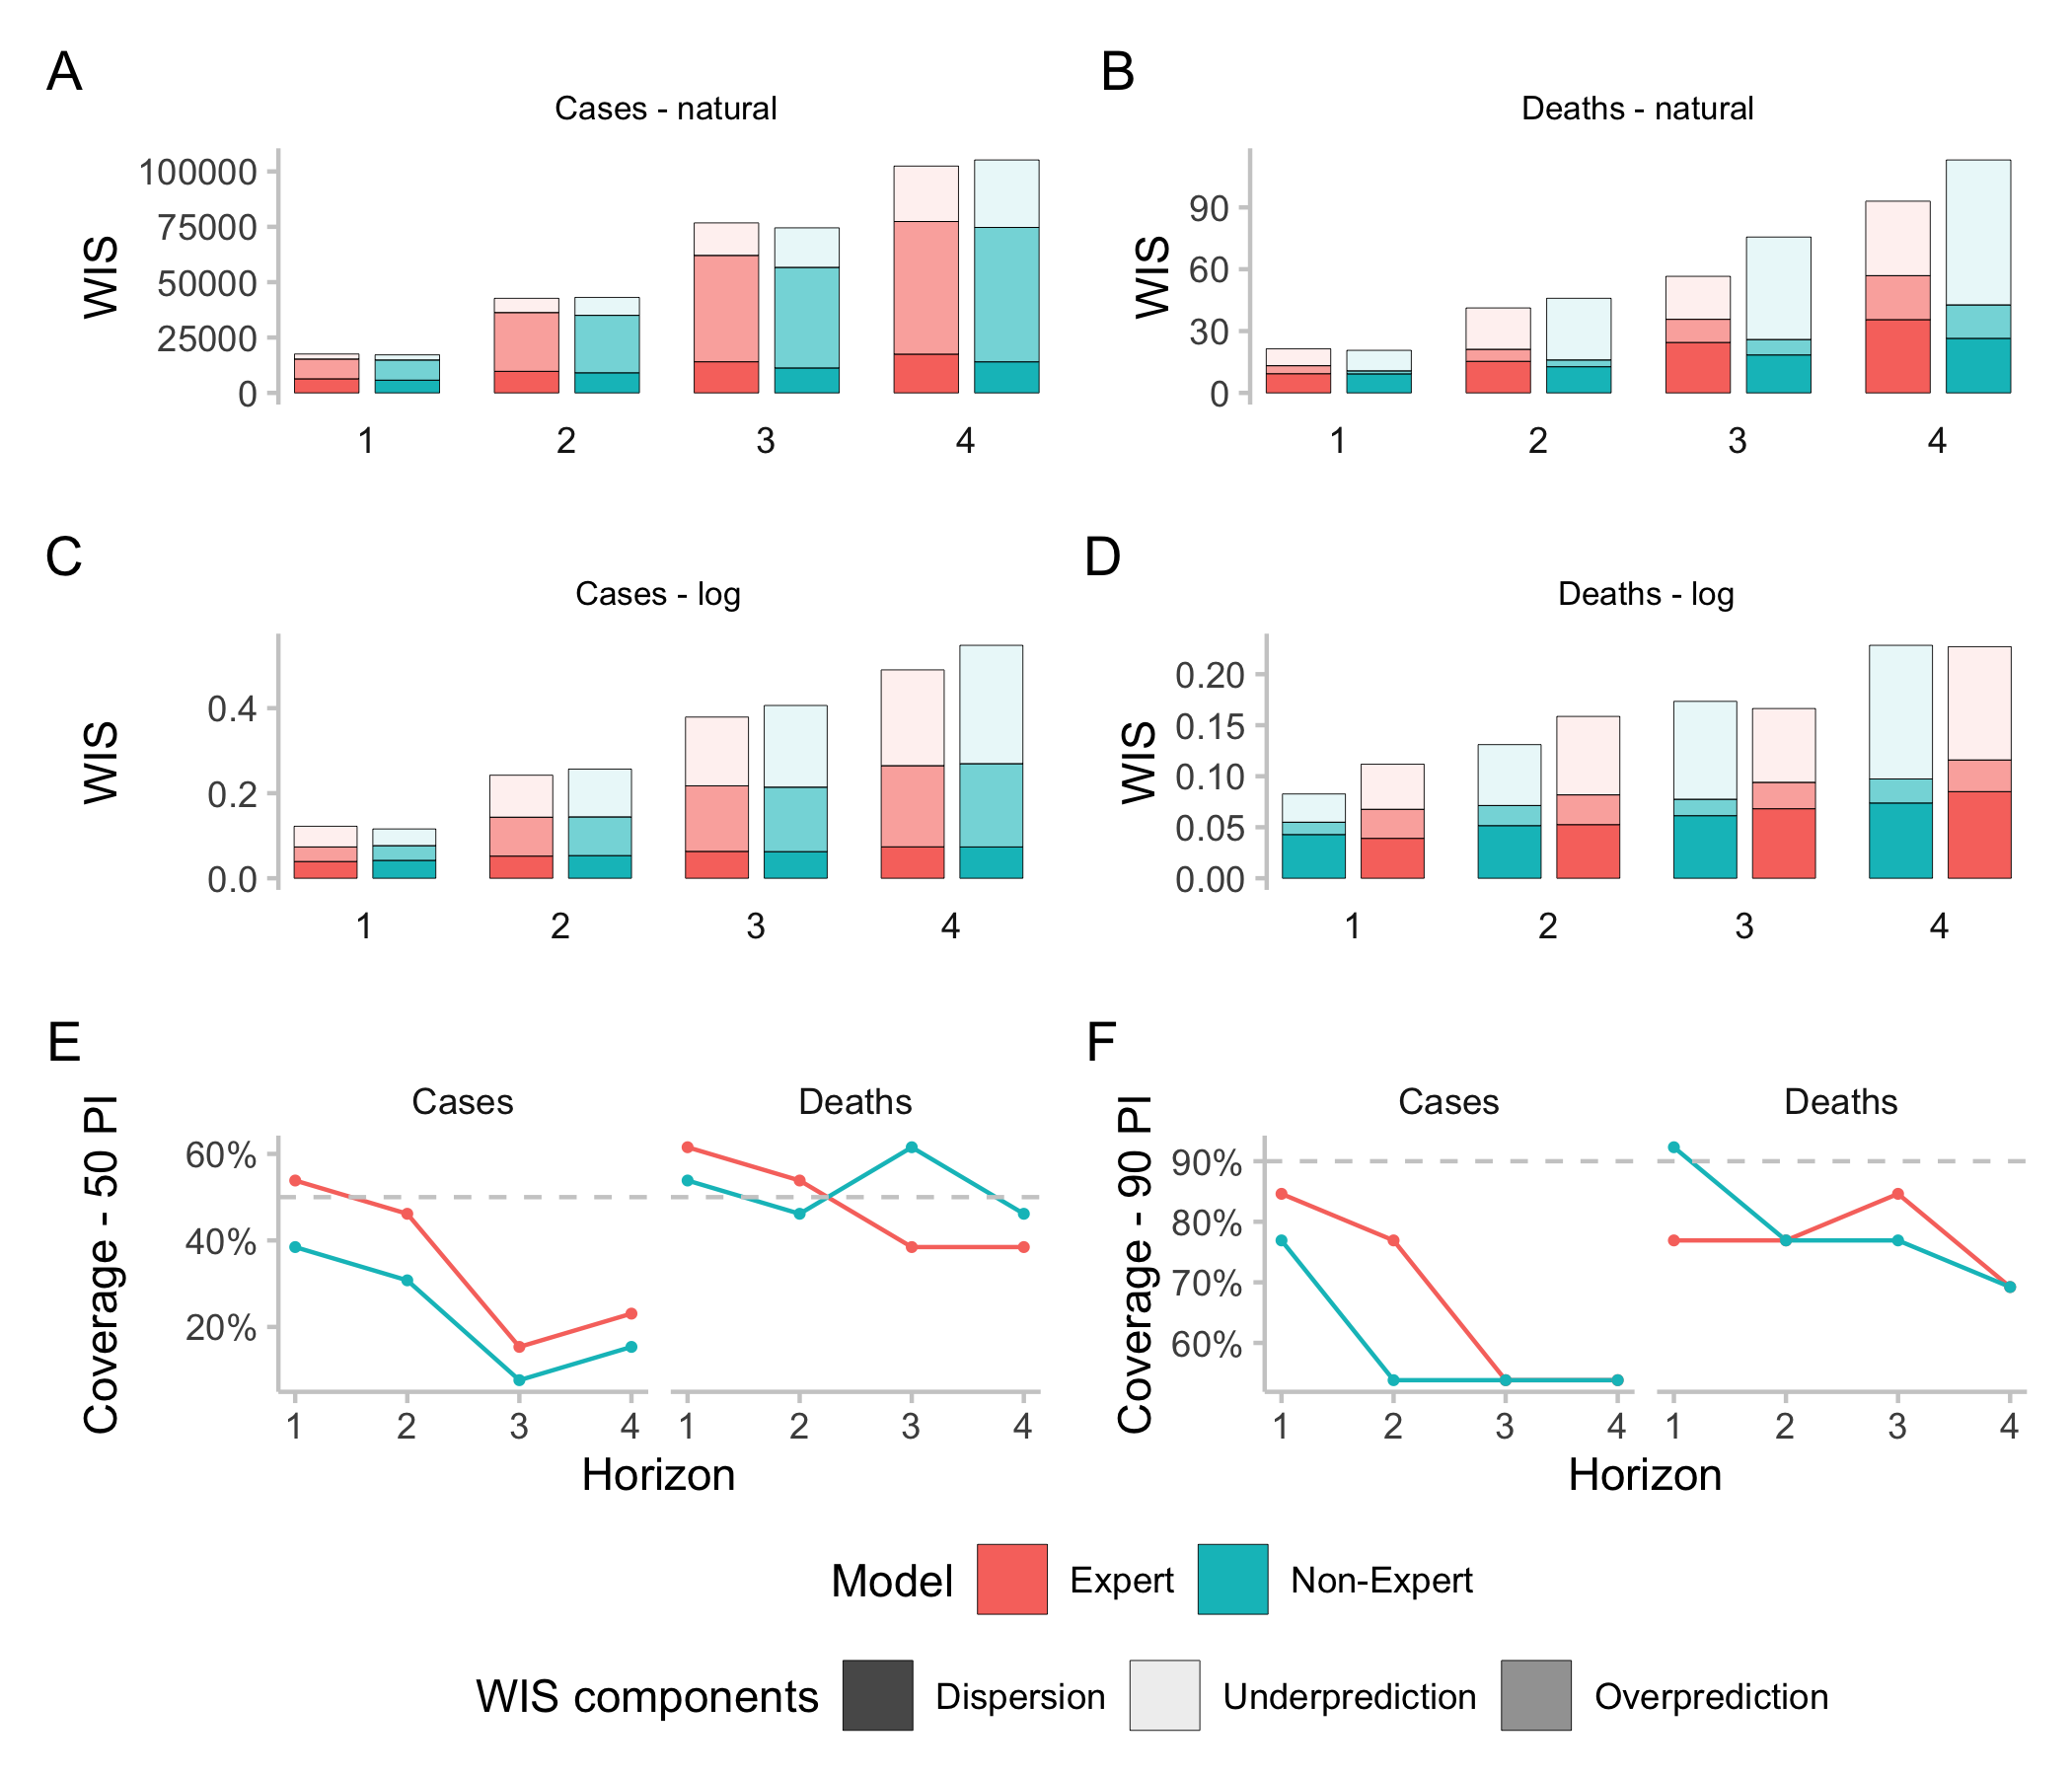
\includegraphics[width=0.99\textwidth]{../output/figures/performance-expert.png}
\caption{\bf{Predictive performance of self-reported "experts" and "non-experts" across forecast horizons.} Forecasts from "experts" and "non-experts" were combined to two separate median ensembles, including both direct and $R_t$ forecasts. A-D: WIS stratified by forecast horizon for cases and deaths on the natural and log scale. E, F: Empirical coverage of the 50\% and 90\% prediction intervals stratified by forecast horizon and target type.}
\label{fig:performance-experts}
\end{figure*}


% See this guide for more information on BibTeX:
% http://libguides.mit.edu/content.php?pid=55482&sid=406343

% For more author guidance please see:
% http://wellcomeopenresearch.org/for-authors/article-guidelines

% When all authors are happy with the paper, use the 
% ‘Submit to WELLCOME OPEN RESEARCH' button from the menu above
% to submit directly to the open life science journal Wellcome Open Research.

% Please note that this template results in a draft pre-submission PDF document.
% Articles will be professionally typeset when accepted for publication.

% We hope you find the Wellcome Open Research Overleaf template useful,
% please let us know if you have any feedback using the help menu above.



\end{document}